\documentclass[]{article}
% ATLAS macros
\usepackage{atlasphysics}
% Nice maths macros
\usepackage{amsmath}
% Feynman diagrams
\usepackage{feynmp}
% Figures and floats
\usepackage{graphicx,subfig,float}

% Graphics folider
\graphicspath{{figures/}}

% Read .1 file extension as .mps.
\DeclareGraphicsRule{.1}{mps}{*}{}

% Scientific notation
% http://www.tapdancinggoats.com/easy-scientific-notation-in-latex.htm
\providecommand{\e}[1]{\ensuremath{\times 10^{#1}}}

\begin{document}

\title{Numerical Evaluation of the $\ee \to \mumu$ Cross Section in the Standard Model}
\author{Alex Pearce}
\date{\today}
\maketitle


\begin{abstract}
The recent discovery of both the $\Wboson$ bosons and the $\Zzero$ boson via the $\antibar{p}$ channel by the Super Proton Synchrotron (SPS) team at CERN (Rubbia, van der Meer et al.~\cite{ref:wpaper,ref:zpaper}) opens up new opportunities for accelerator physics. We performed a numerical integration of the differential cross section of the $\ee \to \mumu$ scattering process with a trapezium and a Monte Carlo algorithm in the hope that the proposed Large Electron-Positron collider (LEP) will verify the existence of this channel of $\Zzero$ production. A large resonance at $\sqrt{s}=91.21\pm0.01\GeV$ was found, slightly above the $\Zzero$ mass. The peak cross section was found to be $\sigma=(5.15\pm0.05)\e{-6}\GeV^{-2}=0.200\pm0.002\mathrm{nb}$. Implementing the algorithms in C was found to be nearly 50 times faster than in Python.
\end{abstract}


\section{Introduction}\label{sec:intro}

The proposition of three mediators of the weak nuclear force, the $\Wplus$, $\Wminus$ and $\Zzero$ bosons, has been proven by the current SPS team at CERN. The suggestion of $\Zzero$ production via electron-positron pairs is now becoming of interest to experimentalists. The process manifests itself by an electron-position pair ($e^{-}e^{+}$) annihilating to produce a muon-antimuon pair ($\mu^{-}\mu^{+}$). The process may be mediated by photons or $\Zzero$ bosons via the electromagnetic and weak interactions respectively. This interaction is described by the Feynman diagram in figure \ref{fig:feynsgammaz}.\footnote{The scattering may also be described by a t-channel diagram (figure \ref{fig:feyntgammaz}), however we proceed by analysing the s-channel as it is only via this channel which we may measure resonances and new unstable particles. Note that a u-channel diagram also exists, but it is merely a swapping of the outgoing particles' momenta in the t-channel. We ignore the u-channel for this reason.}

Feynman diagrams allow us to apply the Feynman rules thus producing a  matrix element $\mathcal{M}$. The square of this matrix element corresponds to a differential cross section $\frac{\d{\sigma}}{\d{\Omega}}$ which may be integrated to find the total cross section $\sigma$, which is measurable by a detector.

The following section briefly outlines the theory behind the interactions. The integration methods used to evaluate the differential cross sections are explored in section \ref{sec:integration}, along with a study of the differential cross sections in order to judge the effectiveness of numerical integration upon them. The results are presented and analysed in section \ref{sec:results}, and a brief discussion on performance is given in section \ref{sec:performance}. Finally, some conclusions are drawn in section \ref{sec:conclusion}.

\section{Principles of Interaction Cross Sections}

With reference to the Feynman diagrams in figures \ref{fig:feynsgammaz} and \ref{fig:feyntgammaz}, the incoming particles are labelled with the four-momenta $p_{1}$ and $p_{2}$, whilst the outgoing particles carry $p_{3}$ and $p_{4}$. Here we have suppressed the four-vector notation, implicitly assuming tensor notation. At LEP, the electrons and positrons will be accelerated around a circular collider in opposite directions. The collider energy is then given by $\sqrt{s}$, where $$s = (p_{1} + p_{2})^{2}.$$

The differential cross sections are dependent on the collider energy via the dimensionless variables $$\varepsilon = \frac{m_{\mu}}{\sqrt{s}}, \quad \lambda = \frac{M_{\Zzero}}{\sqrt{s}},$$ where $m_{\mu}$ is the muon mass and $M_{\Zzero}$ is the $\Zzero$ boson mass. It is worth noting that the energies LEP will be operating at allow us to take the electron as massless in the ultrarelativistic limit.\footnote{In addition the muon is over 200 times more massive than the electron so we may disregard the electron mass in scattering interactions.}

\subsection{Real and Virtual Particles}

As noted in figure \ref{fig:feynsgammaz}, the scattering may be mediated by either a virtual photon $\gamma^{*}$ or a $\Zzero^{(*)}$ boson, where the bracketed star notation indicates that the boson may be either \emph{on-} or \emph{off-mass-shell}. These terms refer to how well the mediating particles (propagators in the Feynman diagrams) adhere to the mass-energy relation $E^{2} - \lvert{\vec{p}}\rvert^{2}c^{2} = m^{2}c^{4}$. Propagators exceeding the `classical' relativistic values of $E$ and $p$ are off-shell, and said to be virtual particles. This violation of relativity is allowed because it is permitted by the Heisenberg uncertainty principle $\Delta E\Delta t \geq \hbar$; the violation in energy may only exist for a very short period of time.

As the $\Zzero$ is an unstable particle it has a finite lifetime. By the uncertainty principle, there is then a range of permitted energies under which the boson will become on-shell. Within this range, we should expect the $\Zzero$ to begin mediating scattering interactions allowing us to detect it via a peak in the cross section $\sigma$. 

\subsection{Differential Cross Sections}

LEP will detect the integrated square of the total matrix element $\mathcal{M}$. As the propagator in the interaction may be one of two particles, $\mathcal{M}$ must be the sum of two separate matrix elements (one matrix element for each possible propagator). The measurable quantity, the cross section $\sigma$, is the integrated square of the total matrix element so we must have the square of a sum:

\begin{align*}
\mathcal{M} &= \mathcal{M}_{\gamma} + \mathcal{M}_{\Zzero},
\\
\mathcal{M}^{2} &= (\mathcal{M}_{\gamma} + \mathcal{M}_{\Zzero})^{2}
\\
&= \mathcal{M}_{\gamma}^{2} + \mathcal{M}_{\Zzero}^{2} + 2\operatorname{Re}(\mathcal{M}_{\gamma}\mathcal{M}_{\Zzero}^{*})
\\
&= \frac{\d{\sigma}}{\d{\Omega}}^{\gamma\operatorname{-}\gamma} +
	\frac{\d{\sigma}}{\d{\Omega}}^{\Zzero\operatorname{-}\Zzero} +
	\frac{\d{\sigma}}{\d{\Omega}}^{\gamma\operatorname{-}\Zzero}
\\
&= \frac{\d{\sigma}}{\d{\Omega}}.
\end{align*}

Each term of $\mathcal{M}^{2}$ corresponds to its own differential cross section: the first for the pure photon process, the second for the pure $\Zzero$ process, and the last for the interference of both processes.

The functional form of each differential cross section is derived by applying the Feynman rules to figure \ref{fig:feynsgammaz}. They are given in appendix \ref{app:differentials}.

Plots of the differentials are given in section \ref{ssec:differentialfigs}. Figures \ref{fig:diffbelow}, \ref{fig:diffexact}, and \ref{fig:diffabove} show a pair of plots for collider energies $\sqrt{s}=$ $3\GeV$, $M_{\Zzero}$ = $91.19\GeV$~\cite{ref:pdg}, and $115\GeV$ respectively. The left-hand figure in each pair shows just the QED differential while the right-hand side figure shows the full Standard Model differential.

The full Standard Model distribution only slightly alters the QED distribution in the low energy regime, namely by introducing a small asymmetry in the quadratic form of the curve. The Standard Model contribution is much more prominent for the $M_{\Zzero}$ regime as, not only does it introduce an asymmetry, it shifts the position of the curve along $\frac{\d{\sigma}}{\d{\Omega}}$ by two orders of magnitude. This should result in a large cross section $\sigma$ around this region.

The Standard Model differential in figure \ref{fig:diffsmabove} has a very different form in the high energy regime whilst also increasing the magnitude of the curve.

Each pair of plots show that the Standard Model contribution tends to increase the cross section of the scattering. In particular, we expect to see a large peak in $\sigma$ close to $M_{\Zzero}$.

\section{Integration of the Differential $\frac{\d{\sigma}}{\d{\Omega}}$}\label{sec:integration}

A common approach to numerically approximating integrals is the trapezium rule. We shall use the trapezium rule and compare it with the more recent Monte Carlo method, whereby random points are sampled and the fraction of those between the curve and the dependent axis is proportional to the area i.e. the integral.

The reasoning behind using two methods of numerical integration is twofold. Firstly, it serves as a consistency check: if at least one method is running incorrectly, the results from each are unlikely to agree with each other. Secondly, evaluating the efficiency of each method may be useful for future analysis of particle interaction cross sections. (Indeed, the information may be useful for analysing any functions of a similar form.)

On this point, it is worth noting that the accuracy of each algorithm will depend largely on the functional form of the differential cross sections. Erratic, non-analytic functions will be poorly suited for trapezium evaluation, while functions with very small variations will result in inaccurate Monte Carlo evaluation. The differential forms are plotted in figures \ref{fig:diffbelow}, \ref{fig:diffexact} and \ref{fig:diffabove}. The impact of these forms on the accuracy of the final results will be analysed in section \ref{sec:results}.

\subsection{Method}\label{ssec:method}

Firstly, we observe that there is no $\phi$ dependence in any of the differential cross sections as in appendix \ref{app:differentials}. This makes the integration over $\phi$ trivial ($0\leq\phi\leq2\pi$), adding a factor of $2\pi$ to cross section $\sigma$. This simplifies the problem significantly as we are now dealing with a one-dimensional integral which permits the use of the trapezium rule.

The integration is over circular polar coordinates and we note that the differential $\sin{\theta}\d{\theta}\d{\phi}$ may be expressed as $\d{(\cos{\theta})}\d{\phi}$, hence we may perform the change of variable $\cos{\theta} \to x$. This changes the limits in $\theta$ to the limits in $x$ $$0 \leq \theta \leq \pi \to -1 \leq x \leq 1.$$ Consequently the random numbers generated for the Monte Carlo integration must be generated between -1 and 1 to provide a uniform distribution in $\cos{\theta}$ rather than $\theta$.

A simple Monte Carlo integration will be performed via~\cite{ref:gjdaniell}$$\int\limits_{a}^{b}f(x)\d{x} \approx \frac{b-a}{N}\sum\limits_{i=1}^{N}f(x_{i}),$$ where $N$ is the number of random points to be sampled and $x_{i}$ is the $i^{\mathrm{th}}$ random number within the limits of integration.

A similarly simple trapezium algorithm is used~\cite{ref:gjdaniell}:$$\int\limits_{a}^{b}f(x)\d{x} \approx \frac{h(f(a) + f(b))}{2} + h\sum\limits_{i=1}^{N-1}f(a+ih),\quad h=\frac{b-a}{N}.$$

$h$ is the trapezium width and $N$ is the number of trapezia used to estimate the integral with.

Both methods are given as approximations but it should be considered that as $N \to \infty$ both methods becomes exact (despite this being impossible to perform computationally).

The number of points to sample or the number of trapezia to use will depend on the computational power and time available, as well as the accuracy and precision desired. The exact values used will be discussed in the following section.

We note that the problem may be tackled in two distinct ways. We may either sum the integrands and integrate the resulting function (method $(\ref{eqn:intsum})$), or we can integrate the differentials and then sum the results (method $(\ref{eqn:sumint})$). We will comment further on this point in section \ref{ssec:interference}.

\begin{equation}\label{eqn:intsum}
\sigma_{\mathrm{total}} =
	\int \left ( \frac{\d{\sigma}}{\d{\Omega}}^{\gamma\operatorname{-}\gamma}
	+ \frac{\d{\sigma}}{\d{\Omega}}^{\Zzero\operatorname{-}\Zzero}
	+ \frac{\d{\sigma}}{\d{\Omega}}^{\gamma\operatorname{-}\Zzero}
	\right )
	\d{\Omega}
\end{equation}

\begin{equation}\label{eqn:sumint}
\sigma_{\mathrm{total}} =
	\int \frac{\d{\sigma}}{\d{\Omega}}^{\gamma\operatorname{-}\gamma}\d{\Omega}
	+ \int \frac{\d{\sigma}}{\d{\Omega}}^{\Zzero\operatorname{-}\Zzero}\d{\Omega}
	+ \int \frac{\d{\sigma}}{\d{\Omega}}^{\gamma\operatorname{-}\Zzero}\d{\Omega}
\end{equation}


\section{Results and Analysis}\label{sec:results}

When numerically integrating the differential cross sections, they were evaluated in collider energy steps of $0.01\GeV$ so as to allow fine detail in the plots and precise readings. $1000$ trapezia were used in the trapezium algorithm and 1000 random points were sampled with the Monte Carlo method. Although it is not the case that $N$ trapezia should produce similarly accurate or precise values as $N$ sampled points, it was found that $N=1000$ for both algorithms allowed for a fast computation of the integrals and consistent results with each other.

The integrated cross section is presented in figures \ref{fig:bothgammagamma} and \ref{fig:bothcombined}. Each plot shows both the trapezium and Monte Carlo integration results, but their correspondence is such that they are almost indistinguishable from one another.

The Monte Carlo cross section shows slight fluctuations on a scale of $10^{-8}\GeV^{-2}$ but its general shape follows that of the trapezium evaluation very well.

\subsection{Resonance}\label{ssec:resonance}

There is a striking resonance around the $\Zzero$ mass $M_{\Zzero}$. There is a cross section peak of around $5\e{-6}\GeV^{-2}$ at collider energy $91.21\GeV$. It is important to note that this is \emph{above} the $\Zzero$ mass of $91.19\GeV$. The explanation for this cannot be found in the $\gamma\operatorname{-}\gamma$ channel as there is clearly no resonance in its cross section (figure \ref{fig:bothgammagamma}); it is due to the Standard Model contributions.

The resonance itself is mostly due to the $\Zzero\operatorname{-}\Zzero$ term. We see a significant increase in the cross section around $M_{\Zzero}$ because it is in this range that the $\Zzero$ boson becomes on-shell, and hence becomes real and therefore detectable. The resonance is our detection of the $\Zzero$ boson mediating the scattering interaction.

Recalling the previously mentioned Heisenberg uncertainty principle, $\Delta E$ is the width of the resonance at half maximum and then $\Delta t = \frac{\hbar}{\Delta E}$ corresponds to the lifetime of the $\Zzero$ boson. A rough reading off of figure \ref{fig:bothfocused} gives $\Delta E = 2.5\pm0.3\GeV$ and therefore $\Delta t = \tau = (2.6\pm0.4)\e{-25} \operatorname{s}$. It is now clear that the parameter $\Gamma_{\Zzero}$ is the resonance width at half maximum and is related to the lifetime of the particle.

Note that, from figure \ref{fig:trapgammaz}, the interference term $\gamma\operatorname{-}\Zzero$ contributes nothing at $M_{\Zzero}$.\footnotemark

\footnotetext{The reason for this is found in the Feynman rule for a boson propagator (using the Feynman diagram in figure \ref{fig:feynsgammaz}). For the $\Zzero$ boson it is proportional to $({s - M_{\Zzero} + i\Gamma_{\Zzero} M_{\Zzero}})^{-1}$. When $\sqrt{s} = M_{\Zzero}$ this propagator term is purely imaginary, hence $\operatorname{Re}(\mathcal{M}_{\Zzero}) = 0 \Rightarrow 2\operatorname{Re}(\mathcal{M}_{\gamma}\mathcal{M}_{\Zzero}^{*}) = 0$~\cite{ref:dgriffiths}.}

\subsection{Interference Term $\gamma\operatorname{-}\Zzero$}\label{ssec:interference}

We see from the trapezium-evaluated interference cross section in figure \ref{fig:trapgammaz} that the contribution at $\sqrt{s}=M_{\Zzero}$ is $0$, but past the $\Zzero$ boson mass the contribution is positive. Thus, the interference terms shifts the resonance to slightly higher energies.

The Monte Carlo integration of $\frac{\d{\sigma}}{\d{\Omega}}^{\gamma\operatorname{-}\Zzero}$ shown in figure \ref{fig:mcgammaz} reveals a spectacular failing of the algorithm. Despite its satisfactory performance evaluating all other cross sections, the algorithm fails on integrating the form of the cross section (shown in figure \ref{fig:diffgammaz}).

We believe that this failing is due to the near-linear form of the integrand. Visual inspection of the curve may conclude that the function is linear, but viewed over a wider range in $\cos{\theta}$ the function is non-linear, resembling a quadratic form. The range $-1\leq\cos{\theta}\leq1$ is tightly zoomed in on a small segment of a curved line and so closely approximates a linear function.

The Monte Carlo approach has great difficulty in accurately evaluating the integral in this case as many sampled points, more than could be available given reasonable time constraints, are required to account for the incredibly subtle functional form. This subtlety results in very erratic behaviour on numerical evaluation, resulting in both inaccurate and inconsistent results. The trapezium rule allows for this subtly, producing consistent results.

The Monte Carlo method's erratic behaviour produces a $\gamma\operatorname{-}\Zzero$ cross section an order of magnitude larger the trapezium result. Due to this, the Monte Carlo resonance peak varies by $\pm0.5\e{-7}\GeV^{-2}$. Its position and value fluctuates around the trapezium peak on subsequent trials.

As touched on in section \ref{ssec:method}, there are two available ways we may evaluate the integrals, methods $(\ref{eqn:intsum})$ and $(\ref{eqn:sumint})$. If we use method $(\ref{eqn:intsum})$, the subtleties of the interference term are absorbed into the other differentials. Integrating the sum therefore eliminates the only major problem we encountered when using the Monte Carlo algorithm. The trapezium rule was invariant in both performance and results with respect to each method.

\subsection{Results}\label{ssec:results}


Taking the above in to consideration, we combined the stability of the trapezium evaluation and the fluctuations of  the Monte Carlo evaluation to present a peak resonance of $\sigma=(5.15\pm0.05)\e{-6}\GeV^{-2}=0.200\pm0.002\mathrm{nb}$ at a collider energy of $\sqrt{s}=91.21\pm0.01\GeV$. The integrations were performed under method $(\ref{eqn:intsum})$ with a Monte Carlo standard deviation in the cross section of $20\mathrm{pb}$ and in the collider energy of $0.085\GeV$.

\section{Performance}\label{sec:performance}

Although the trapezium and Monte Carlo methods of numerical integration produced similarly accurate results in negligibly different times, it should be possible to evaluate the integrals quicker.

The reasoning behind this claim is that we have used Python, a scripting language, to solve the problem. Python is generally slower than compiled languages such as FORTRAN or C.

In order to measure any benefits that a compiled language might bring, the Python script was timed over several runs of numerically integrating then summing the separate differential cross sections via the trapezium rule. This time was averaged to give an approximate runtime estimate.

The parameters used were a collider energy running from $3\GeV$ to $200\GeV$ in steps of $0.1\GeV$. The number of trapezia used was $1000$.

After 50 runs of the Python script, the average runtime was $18.7 \pm 0.2 \operatorname{s}$.

A C script was then written which performed the same numerical integrations as the Python script, and again was ran 50 times to find an average runtime. It was found that the C script took an average of $0.40 \pm 0.1 \operatorname{s}$. A plot of the data produced by the C script is given in figure \ref{fig:cboth}. It shows that each script produces comparable results.

The timings show a large difference in performance between the two languages. The C script ran in $2.1\pm0.1\%$ of the time the Python script required.

The program is extremely repetitive; the parameters given above require close to $2$ million iterations of the integration algorithm. The C compiler's ability to make optimisations in the script save small amounts of time per iteration, which are compounded to produce vast improvements in the total runtime.

Using the Python script, summing the individual integrals takes an almost-equal execution time as summing the integrands and then integrating. Interestingly, the C script takes $0.03\pm0.01\operatorname{s}$ less to sum the integrands.

\section{Conclusions}\label{sec:conclusion}

A numerical integration of the $\ee \to \mumu$ scattering cross section was performed in order to analyse its behaviour over a range of collider energies. A resonant behaviour was found near the $\Zzero$ boson mass. Both algorithms performed well, integrating the differentials quickly and accurately, although the Monte Carlo algorithm required substantially more computations to achieve similar precision to the trapezium rule. In order to overcome the subtly in the interference differential cross section, integrating the sum of the differentials is the better approach for Monte Carlo evaluation. The trapezium rule proved to be the more efficient algorithm in this one dimensional case. In higher order problems, the Monte Carlo approach must be carefully analysed to ensure accurate results. Finally, using C produced drastically faster results than when using Python. Using C also allowed a noticeable speed improvement when integrating the sum of the integrands, rather than summing the integrated differentials.

\section{Figures}

\subsection{Feynman Diagrams}

\begin{figure}[H]
	\vspace{10pt}
	% Diagram unit length.
	\unitlength = 1mm
	\centering
	\subfloat[s-channel]{
		\label{fig:feynsgammaz}
		\begin{fmffile}{sgammazcrossing}
		  \begin{fmfgraph*}(40,25)
		    \fmfleft{i1,i2}
		    \fmfright{o1,o2}
		    \fmflabel{$e^{+}, p_{2}$}{i1}
		    \fmflabel{$e^{-}, p_{1}$}{i2}
		    \fmflabel{$\mu^{+}, p_{4}$}{o1}
		    \fmflabel{$\mu^{-}, p_{3}$}{o2}
		    \fmf{fermion}{i2,v1,i1}
		    \fmf{fermion}{o1,v2,o2}
		    \fmf{photon,label=$\gamma^{*}/\Zzero^{(*)}$}{v1,v2}
		  \end{fmfgraph*}
		\end{fmffile}
	}
	\qquad\qquad
	\subfloat[t-channel]{
		\label{fig:feyntgammaz}
		\begin{fmffile}{tgammazcrossing}
		  \begin{fmfgraph*}(40,25)
		    \fmfleft{i1,i2}
		    \fmfright{o1,o2}
		    \fmflabel{$e^+, p_{2}$}{i1}
		    \fmflabel{$e^-, p_{1}$}{i2}
		    \fmflabel{$\mu^+, p_{4}$}{o1}
		    \fmflabel{$\mu^-, p_{3}$}{o2}
		    \fmf{fermion}{o1,v1,i1}
		    \fmf{fermion}{i2,v2,o2}
		    \fmf{photon,label=$\gamma^{*}/\Zzero^{(*)}$}{v1,v2}
		  \end{fmfgraph*}
		\end{fmffile}
	}
	\caption{$e^{-}e^{+}\to\mu^{-}\mu^{+}$ scattering via two different channels. Time flows from left to right.}
\end{figure}

\subsection{Differential Cross Sections}\label{ssec:differentialfigs}

This subsection contains plottings of the QED differential cross section ($\gamma\operatorname{-}\gamma$ channel) and then the full Standard Model cross section ($\gamma\operatorname{-}\gamma$, $\Zzero\operatorname{-}\Zzero$ and $\gamma\operatorname{-}\Zzero$ channels) at three different collider energies.

\begin{figure}[H]
	\vspace{10pt}
	\centering
	\subfloat[QED]{
		\label{fig:diffqedbelow}
		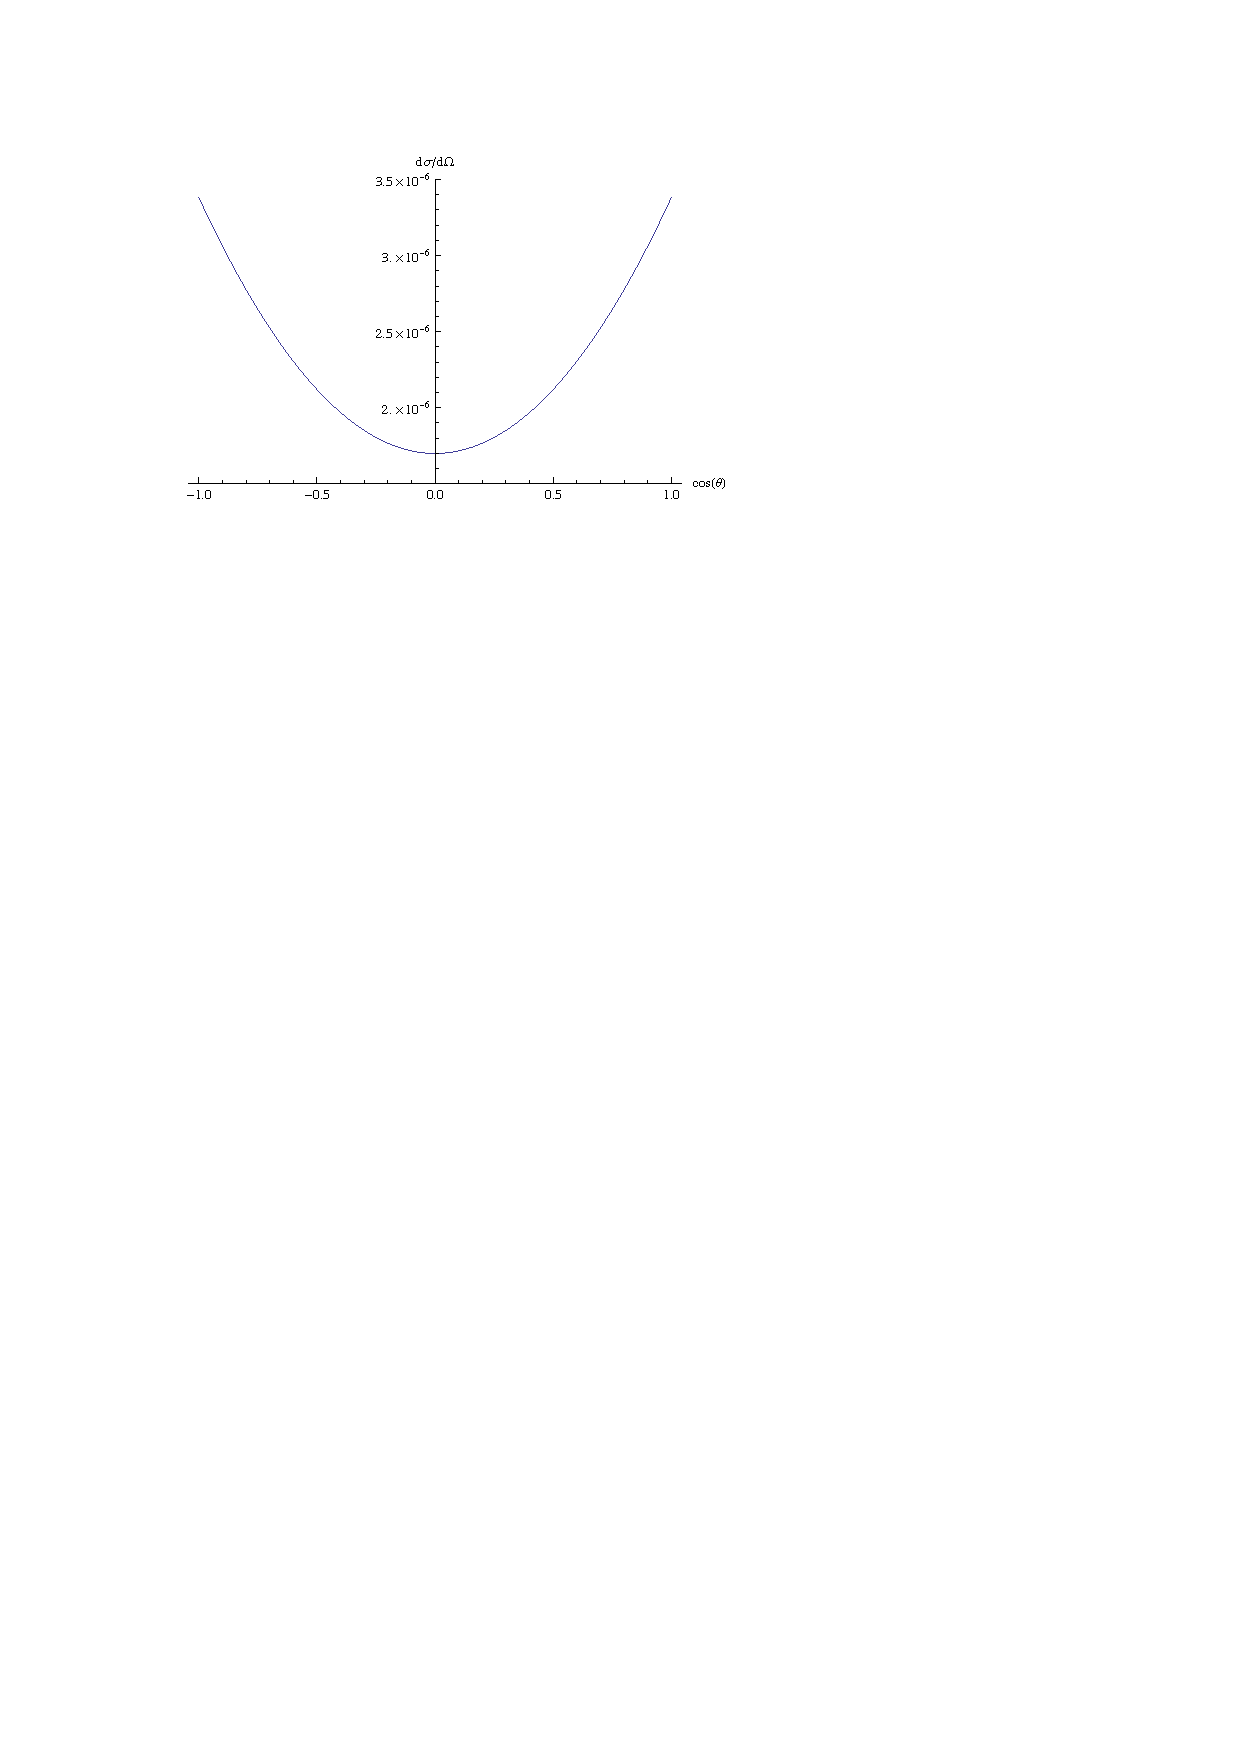
\includegraphics[scale=0.7]{qed_below}
	}
	\subfloat[SM]{
		\label{fig:diffsmbelow}
		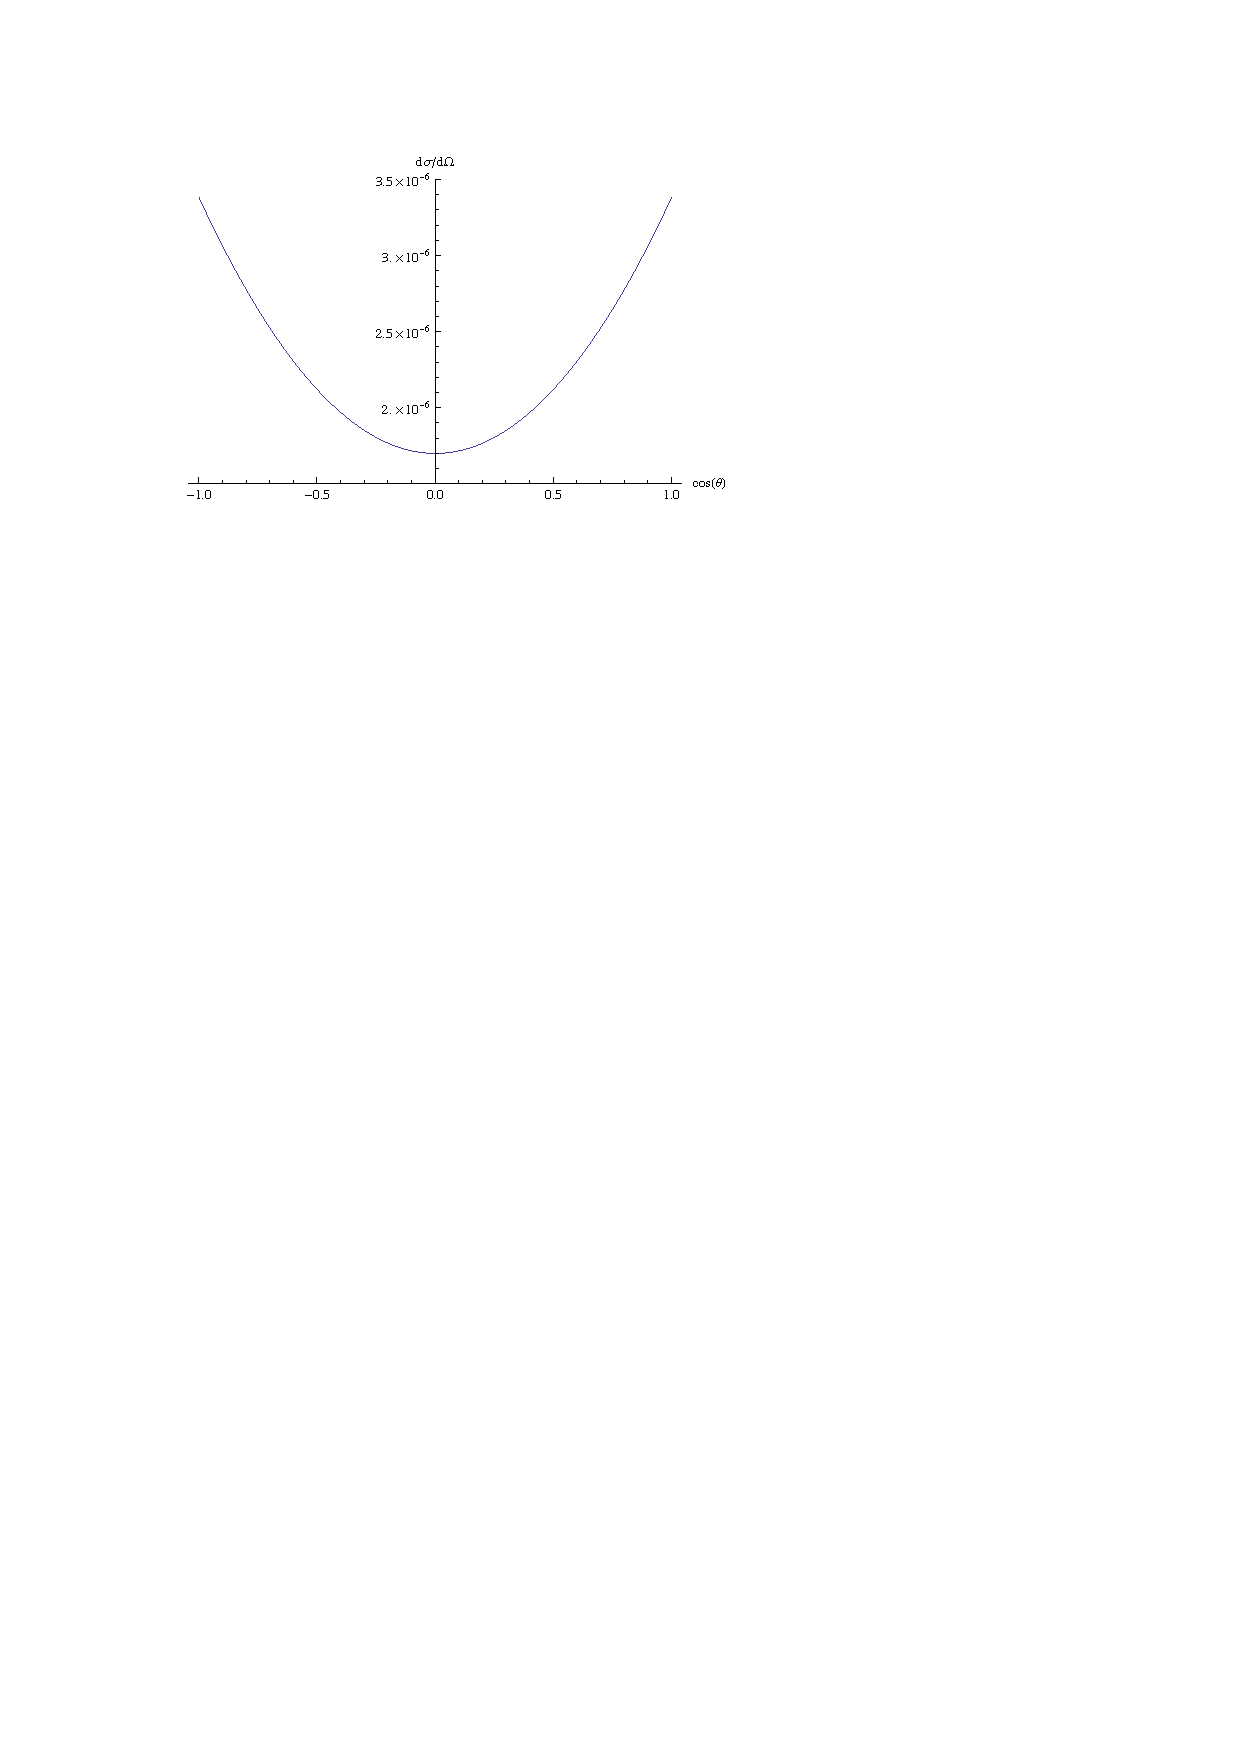
\includegraphics[scale=0.7]{sm_below}
	}
	\caption{$\frac{\d{\sigma}}{\d{\Omega}}$ at $\sqrt{s}=3\GeV$.}
	\label{fig:diffbelow}
\end{figure}

\begin{figure}[H]
	\vspace{10pt}
	\centering
	\subfloat[QED]{
		\label{fig:diffqedexact}
		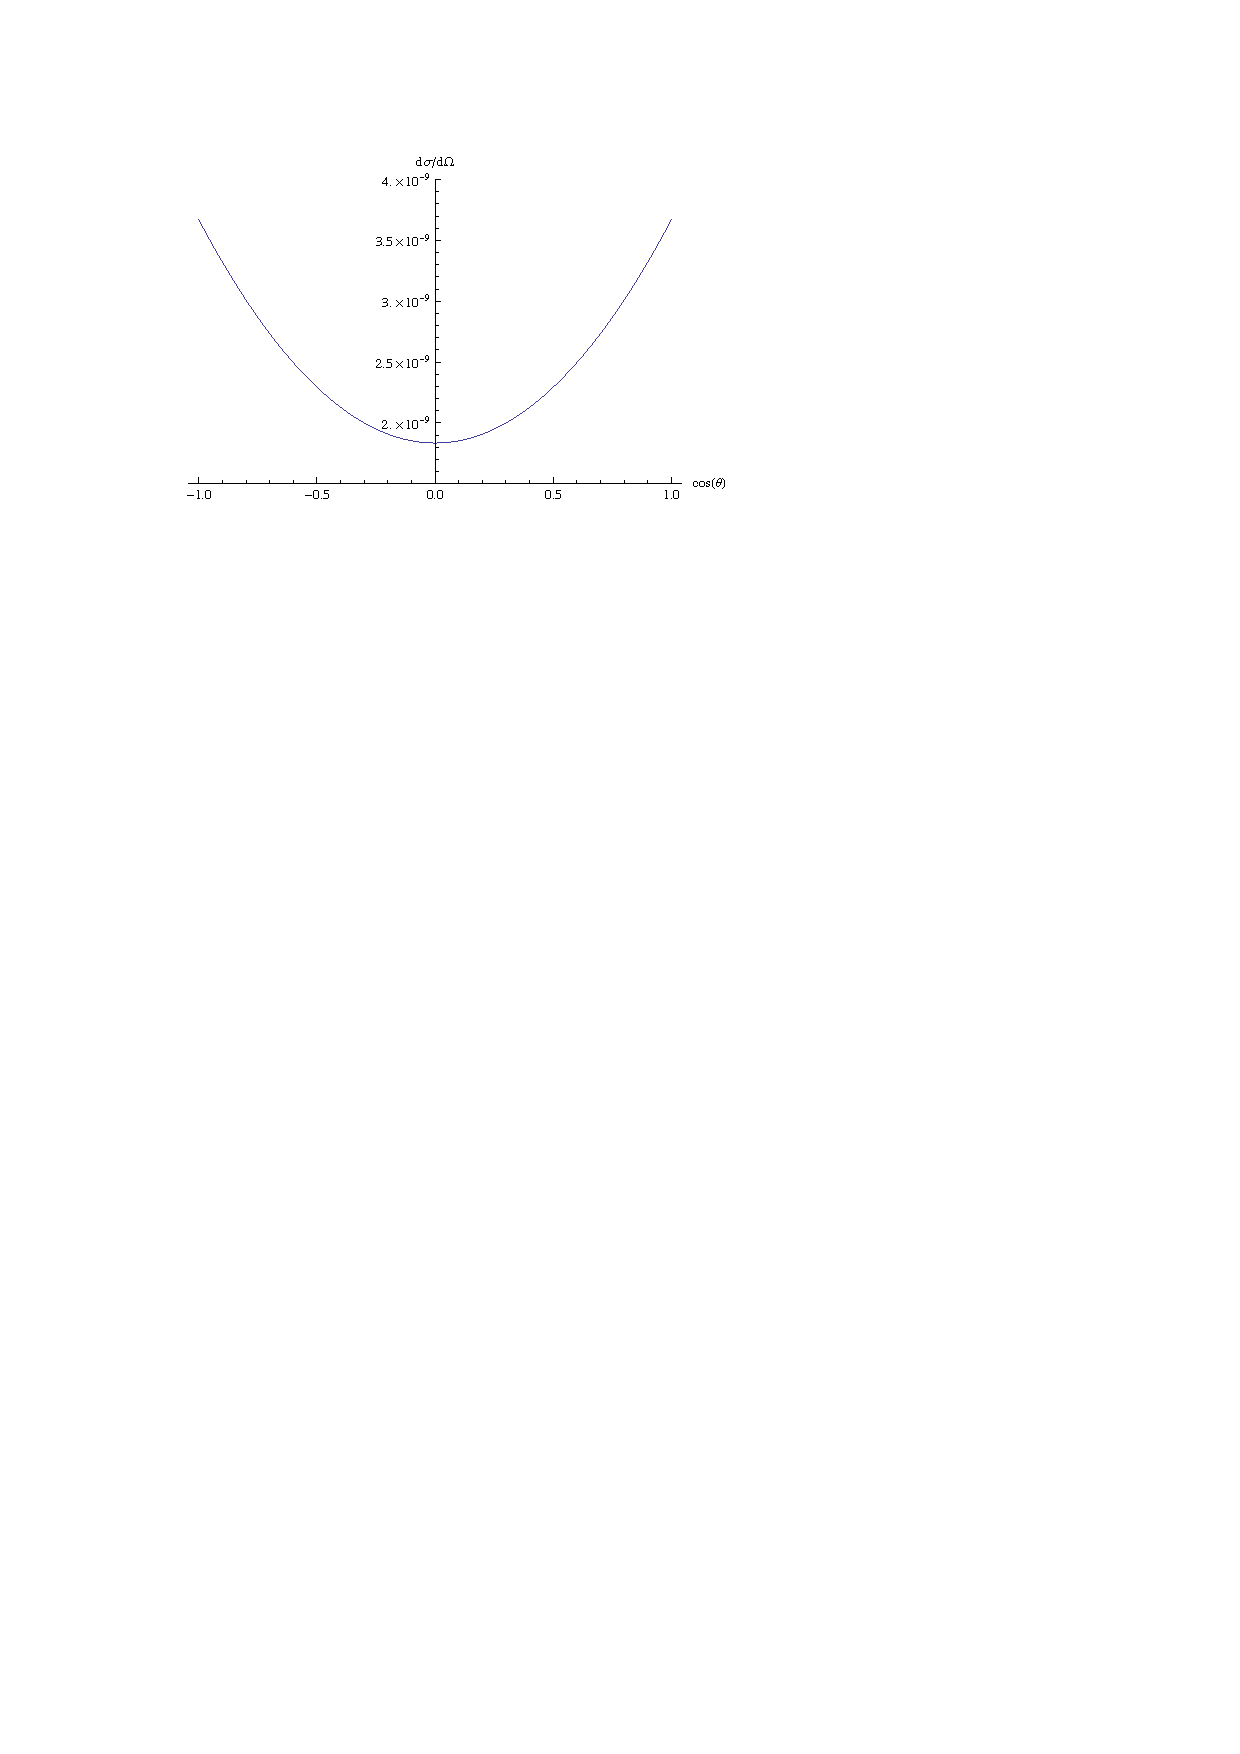
\includegraphics[scale=0.7]{qed_exact}
	}
	\subfloat[SM]{
		\label{fig:diffsmexact}
		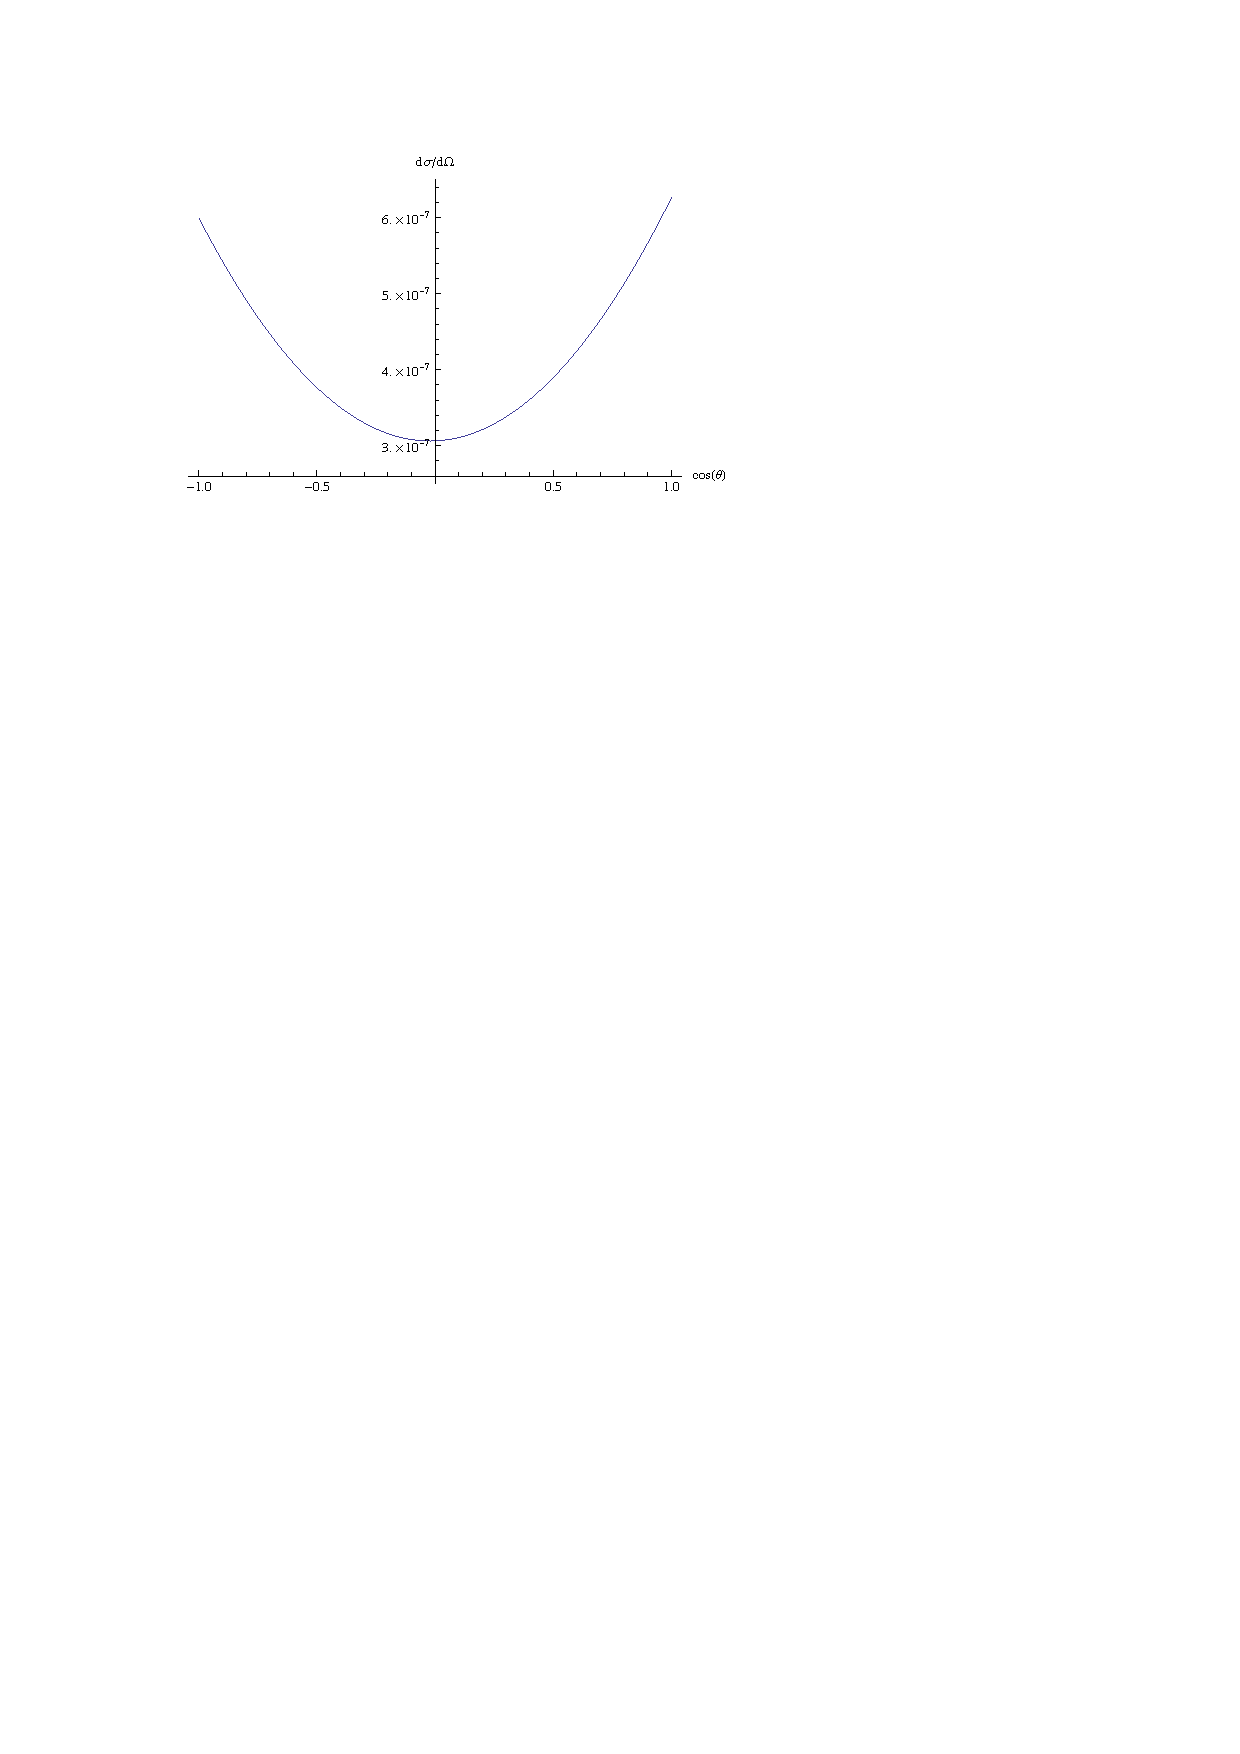
\includegraphics[scale=0.7]{sm_exact}
	}
	\caption{$\frac{\d{\sigma}}{\d{\Omega}}$ at $\sqrt{s}=M_{\Zzero}=91.19\GeV$.}
	\label{fig:diffexact}
\end{figure}

\begin{figure}[H]
	\vspace{10pt}
	\centering
	\subfloat[QED]{
		\label{fig:diffqedabove}
		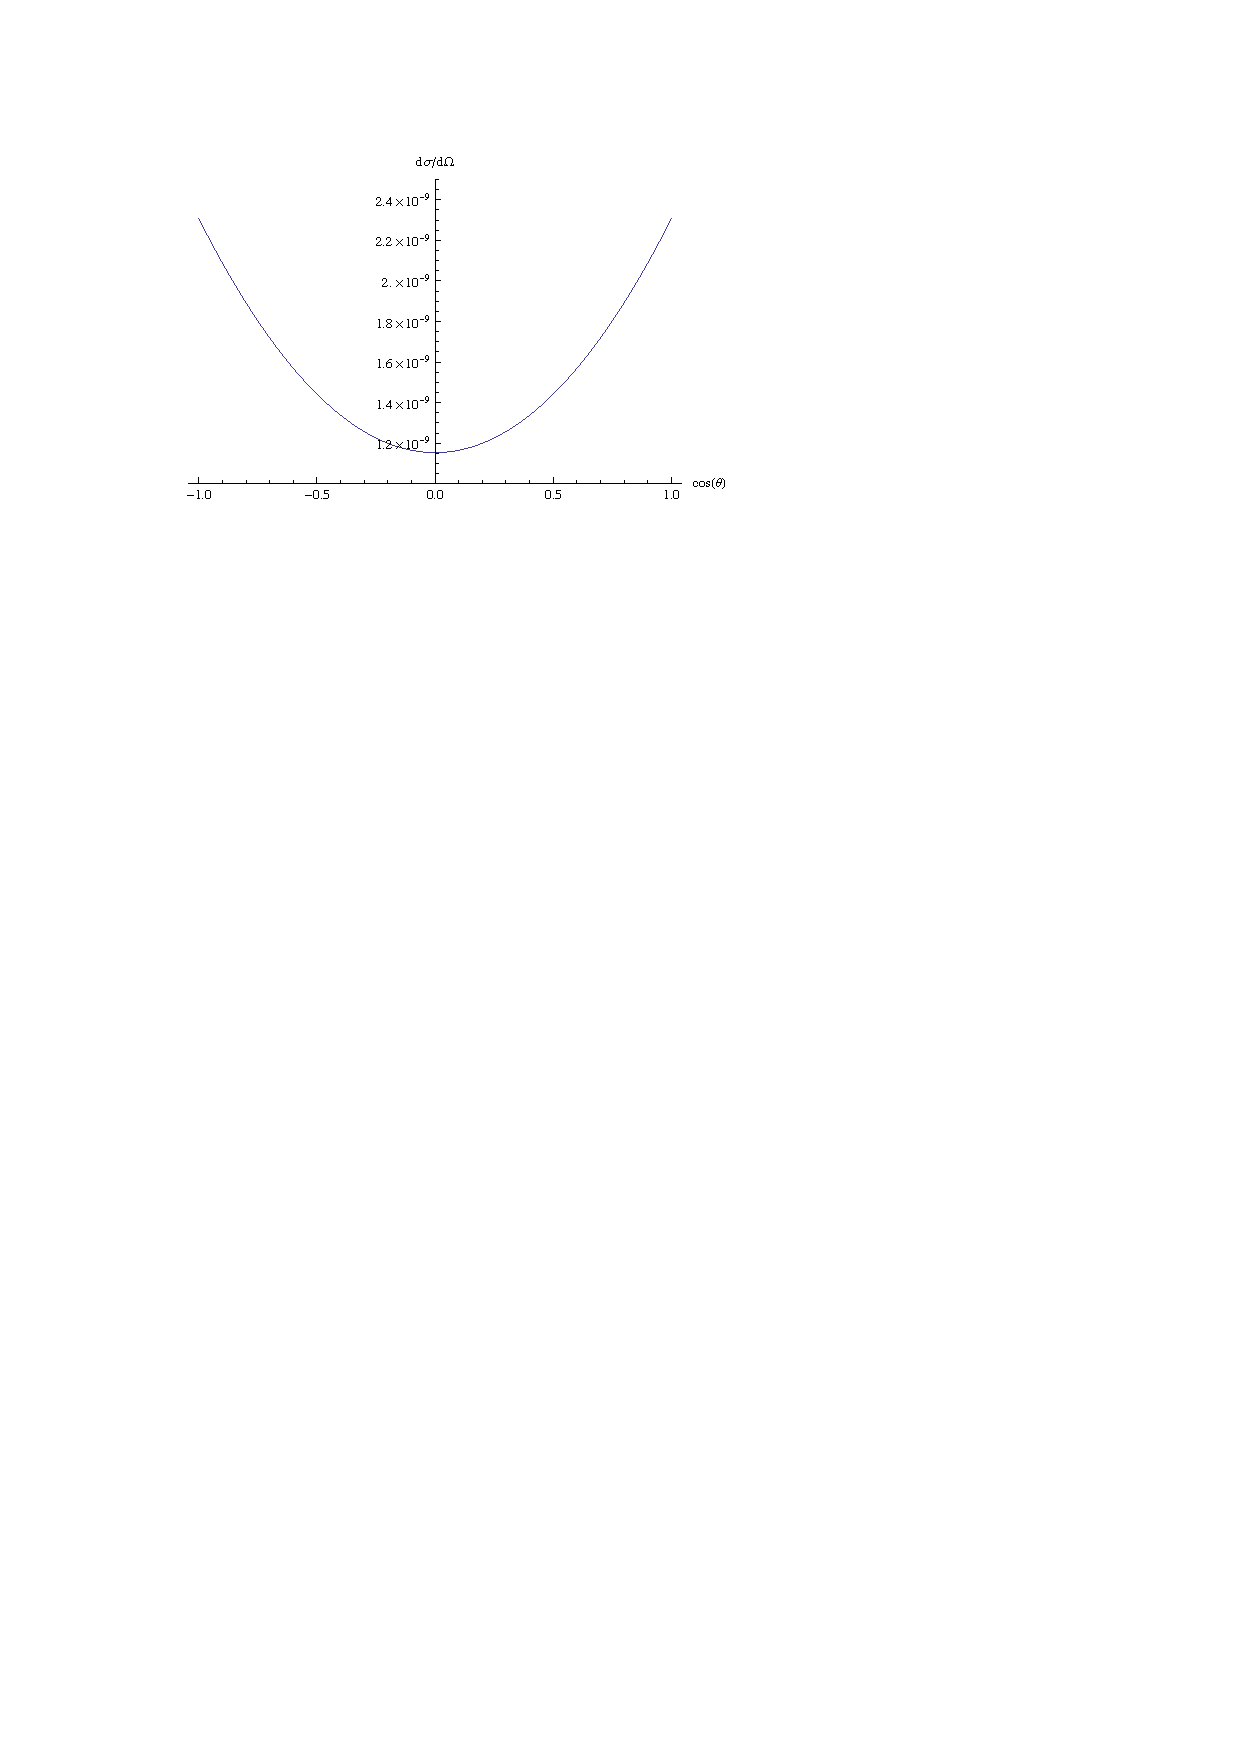
\includegraphics[scale=0.7]{qed_above}
	}
	\subfloat[SM]{
		\label{fig:diffsmabove}
		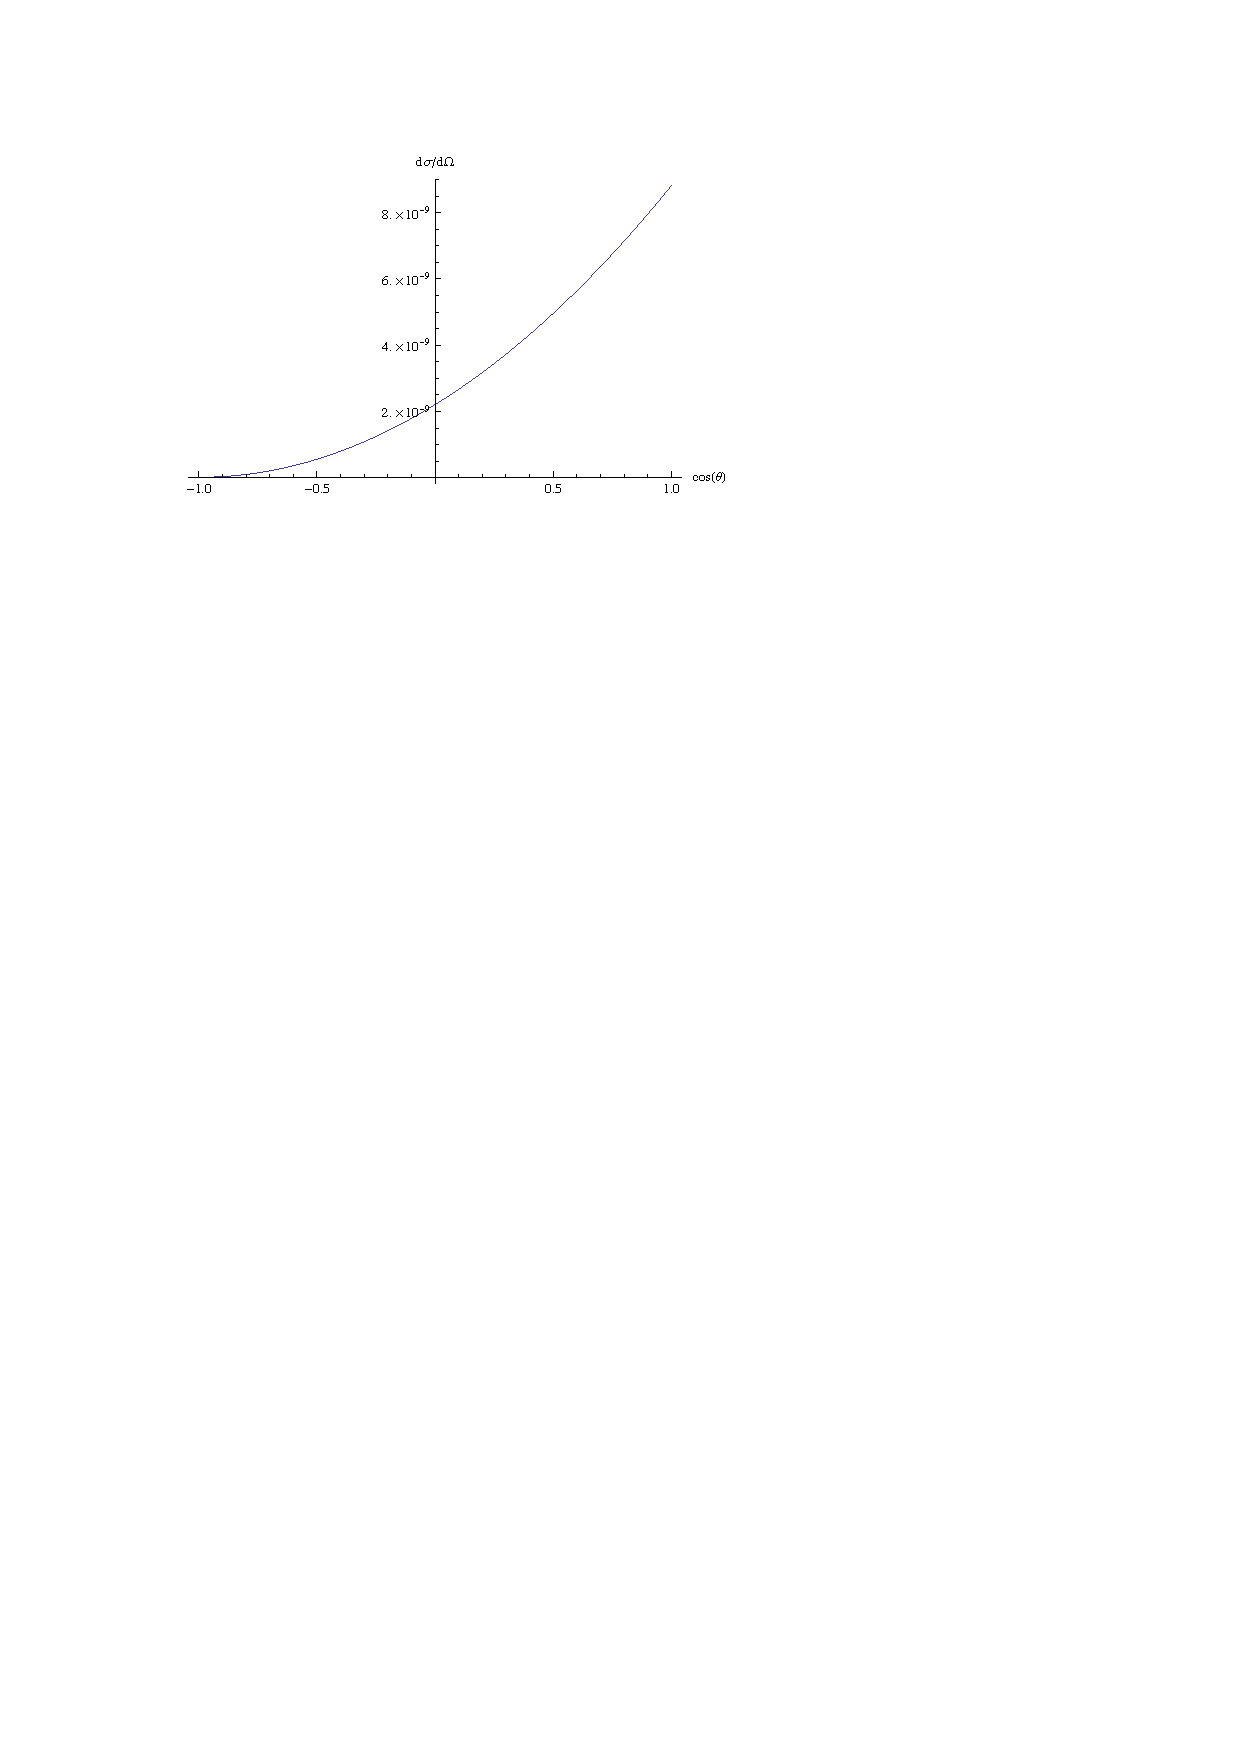
\includegraphics[scale=0.7]{sm_above}
	}
	\caption{$\frac{\d{\sigma}}{\d{\Omega}}$ at $\sqrt{s}=115\GeV$.}
	\label{fig:diffabove}
\end{figure}

\begin{figure}[H]
	\vspace{10pt}
	\centering
	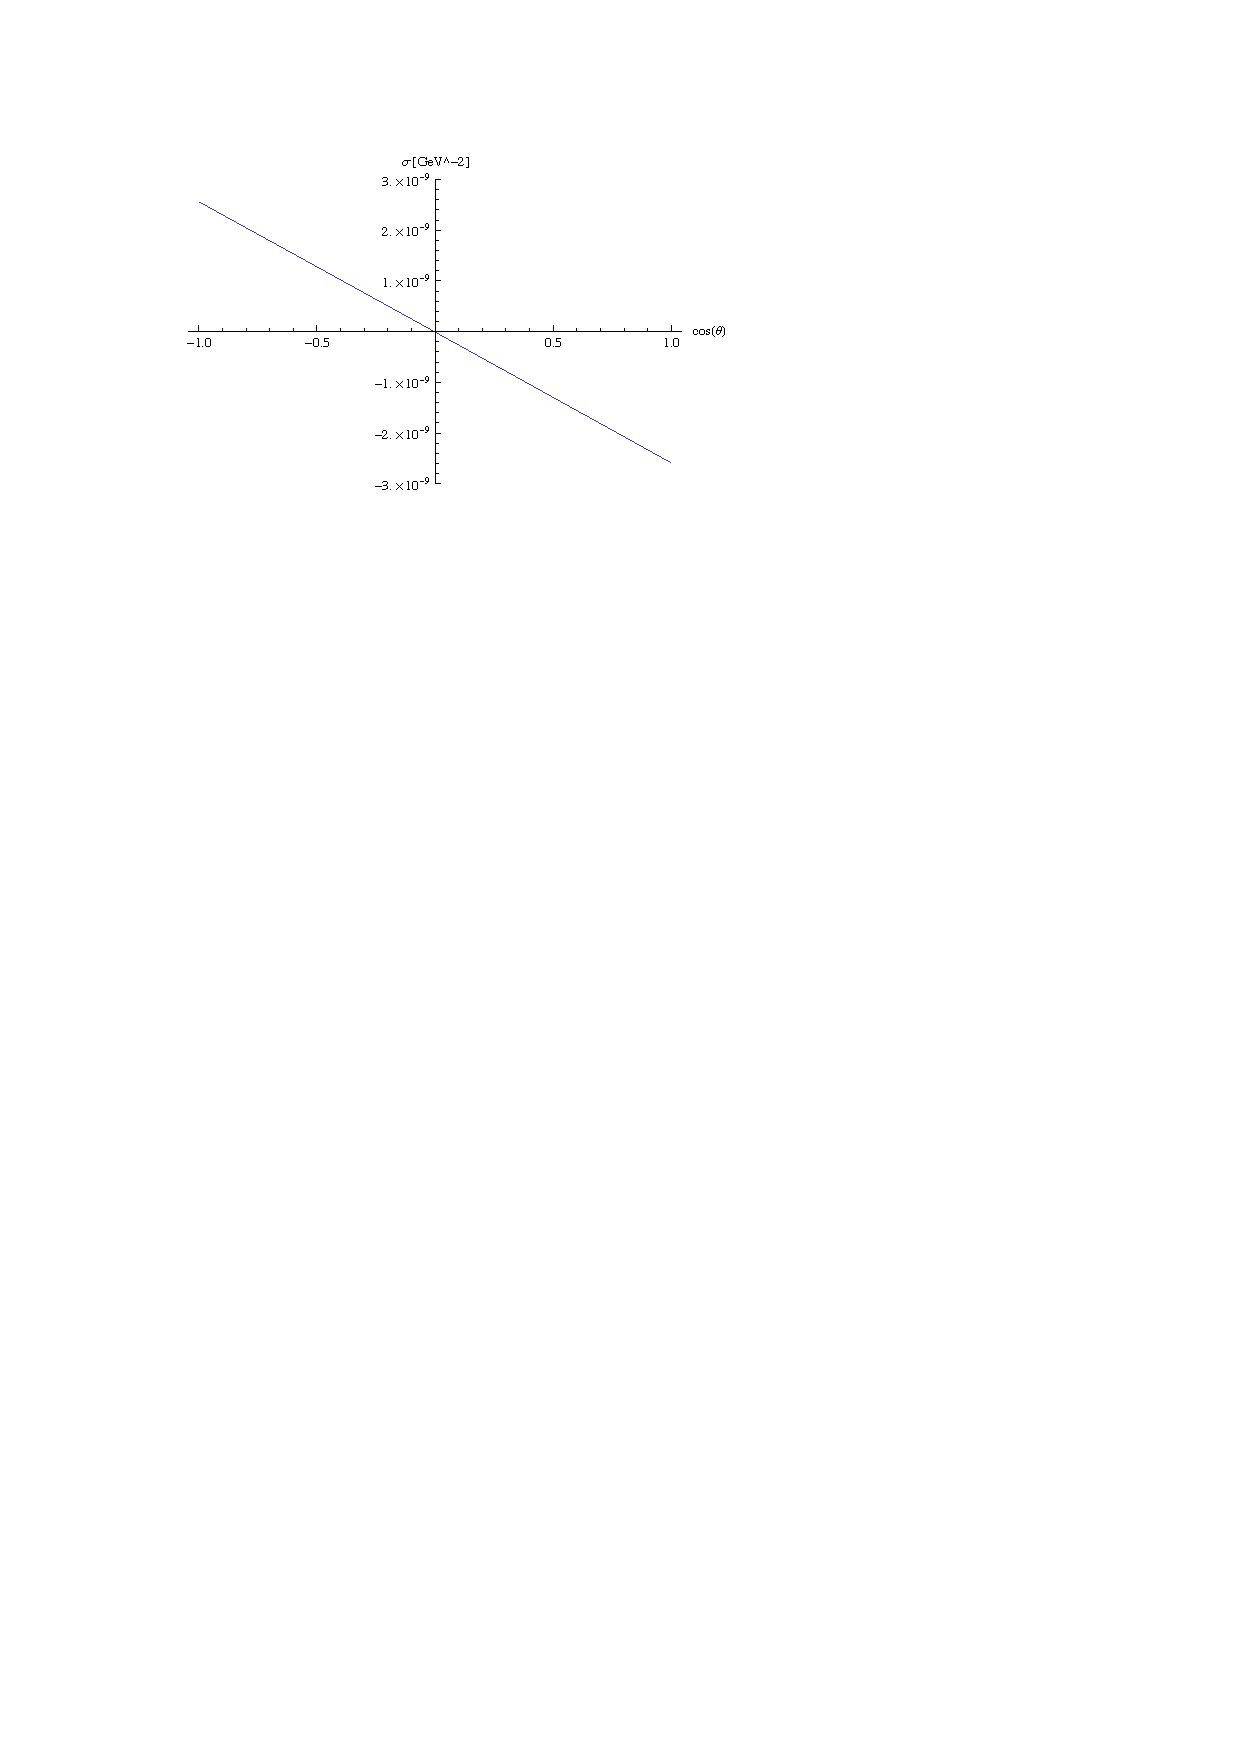
\includegraphics[scale=1.4]{diff_gamma_z}
	\caption{$\frac{\d{\sigma}}{\d{\Omega}}^{\gamma\operatorname{-}\Zzero}$ at $\sqrt{s}=3\GeV$. This extremely linear form is characteristic of the differential also at higher energies.}
	\label{fig:diffgammaz}
\end{figure}


\subsection{Cross Sections $\sigma$}

The following cross sections omit the $2\pi$ prefactor.

\begin{figure}[H]
	\vspace{10pt}
	\centering
	\subfloat[QED]{
		\label{fig:bothgammagamma}
		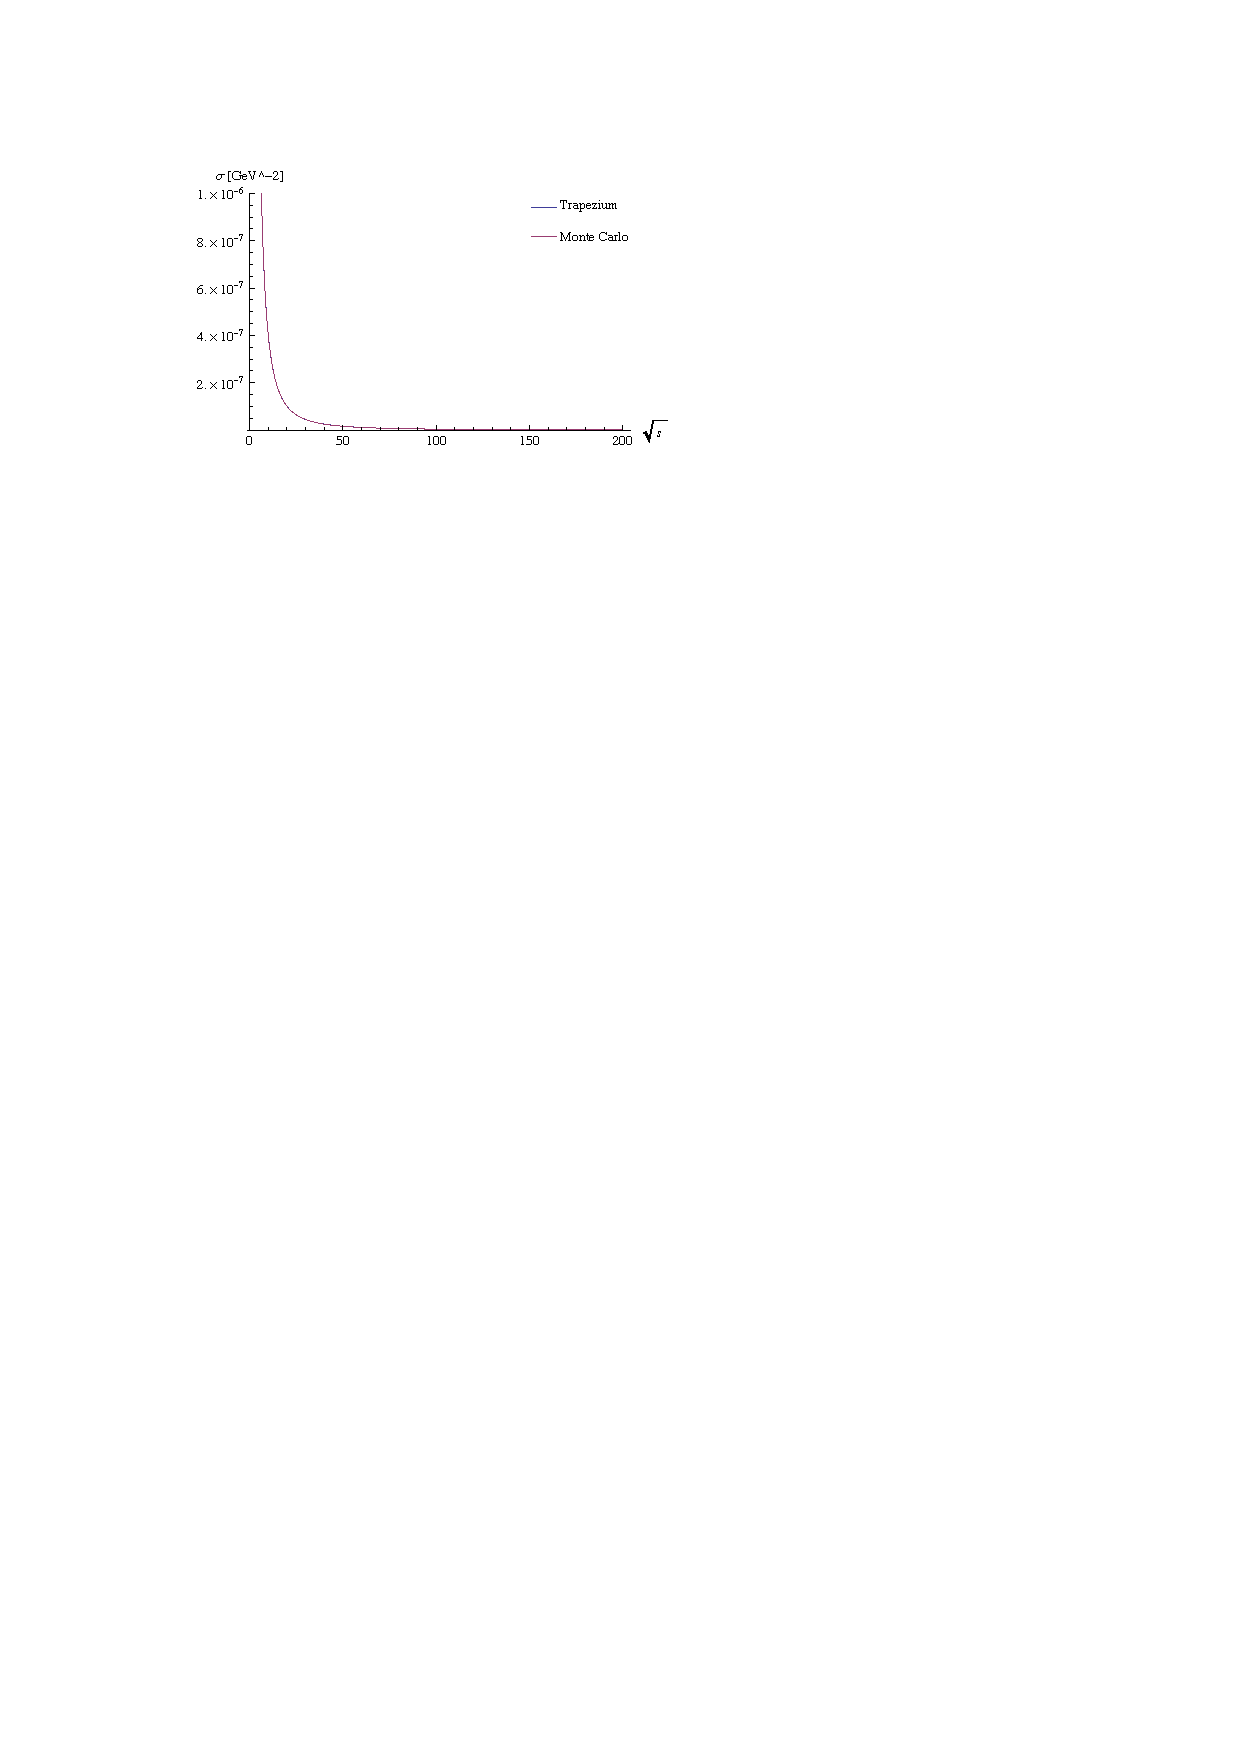
\includegraphics[width=\textwidth]{both_gamma_gamma}
	}\\
	\subfloat[SM]{
		\label{fig:bothcombined}
		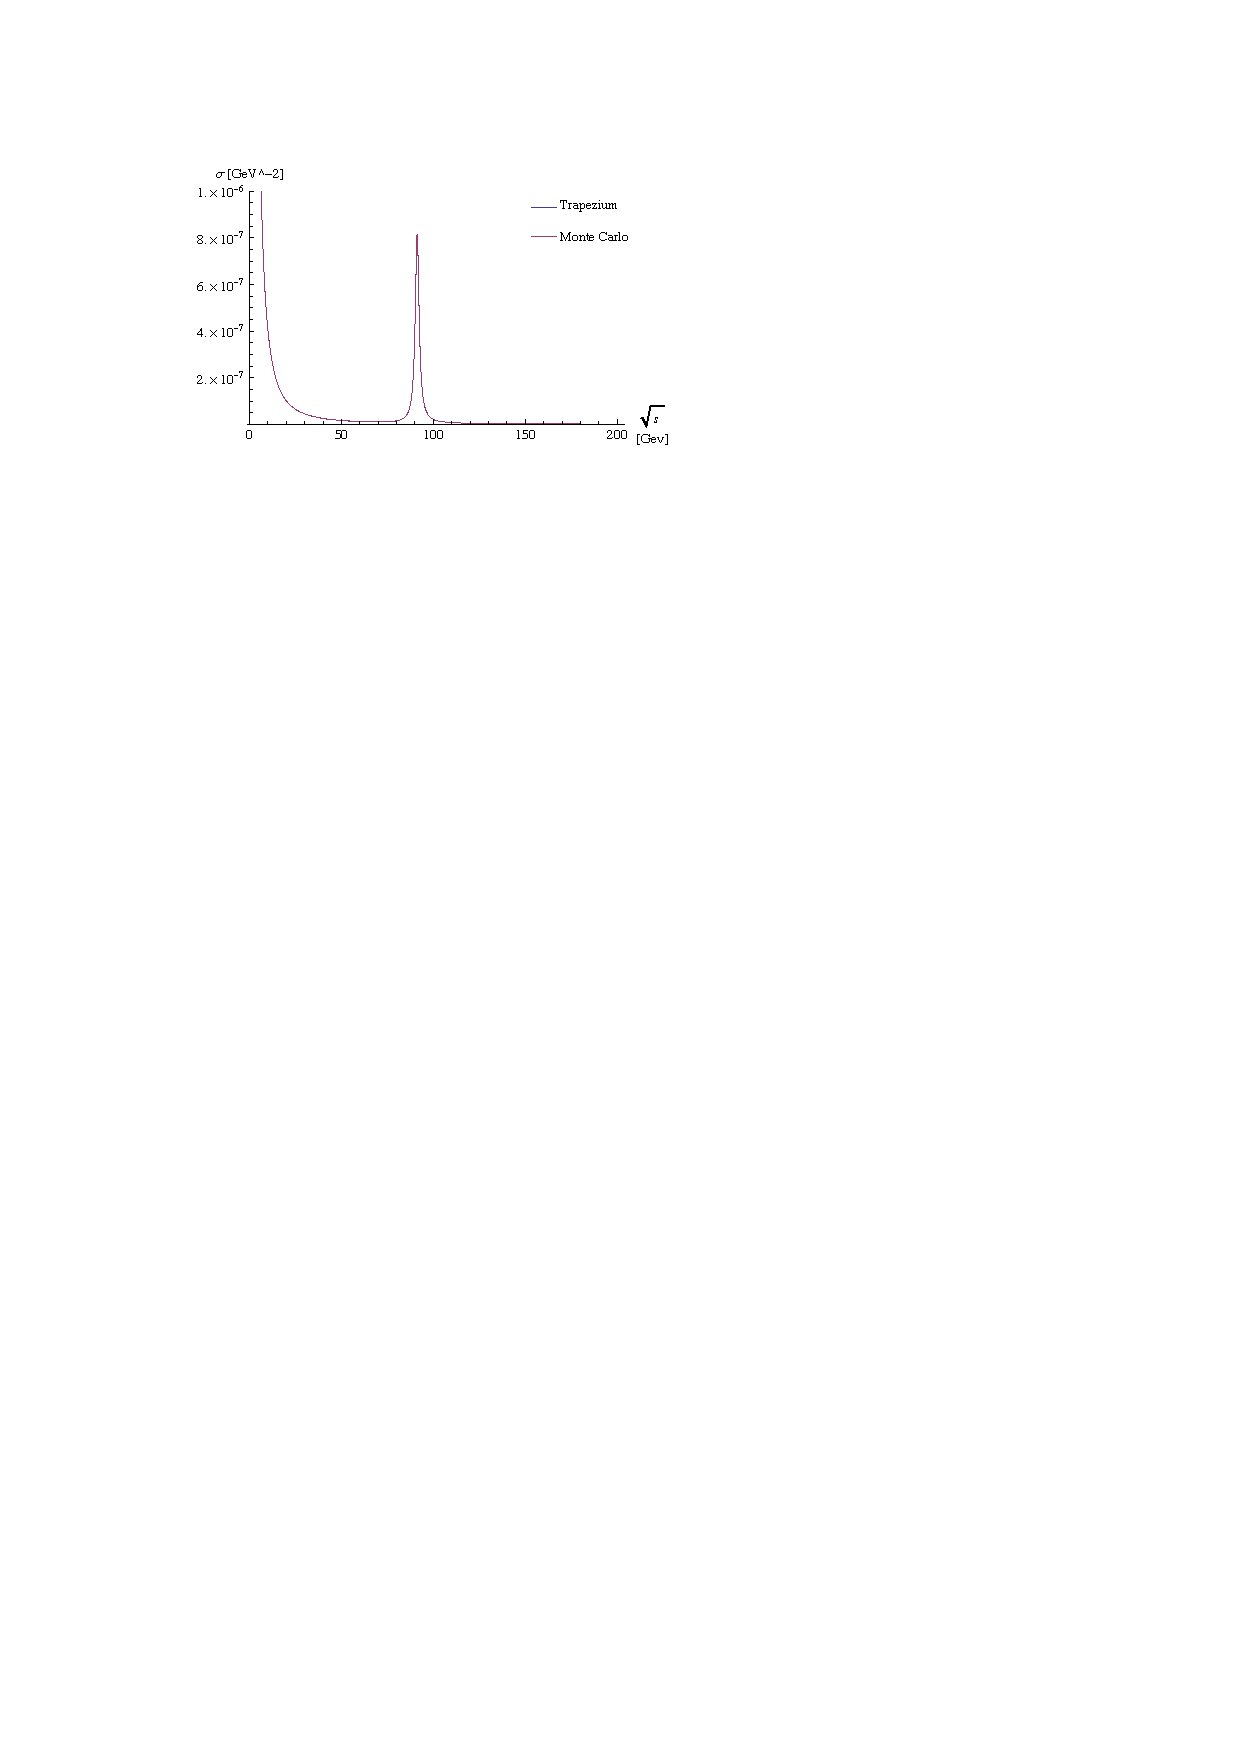
\includegraphics[width=\textwidth]{both_combined}
	}
	\caption{Trapezium and Montecarlo cross section $\sigma$ for collider energies $3\operatorname{-}200\GeV$.}
	\label{fig:both}
\end{figure}

\begin{figure}[H]
	\vspace{10pt}
	\hspace*{-0.1\textwidth}
	\centering
	\label{fig:bothcombinedfocused}
	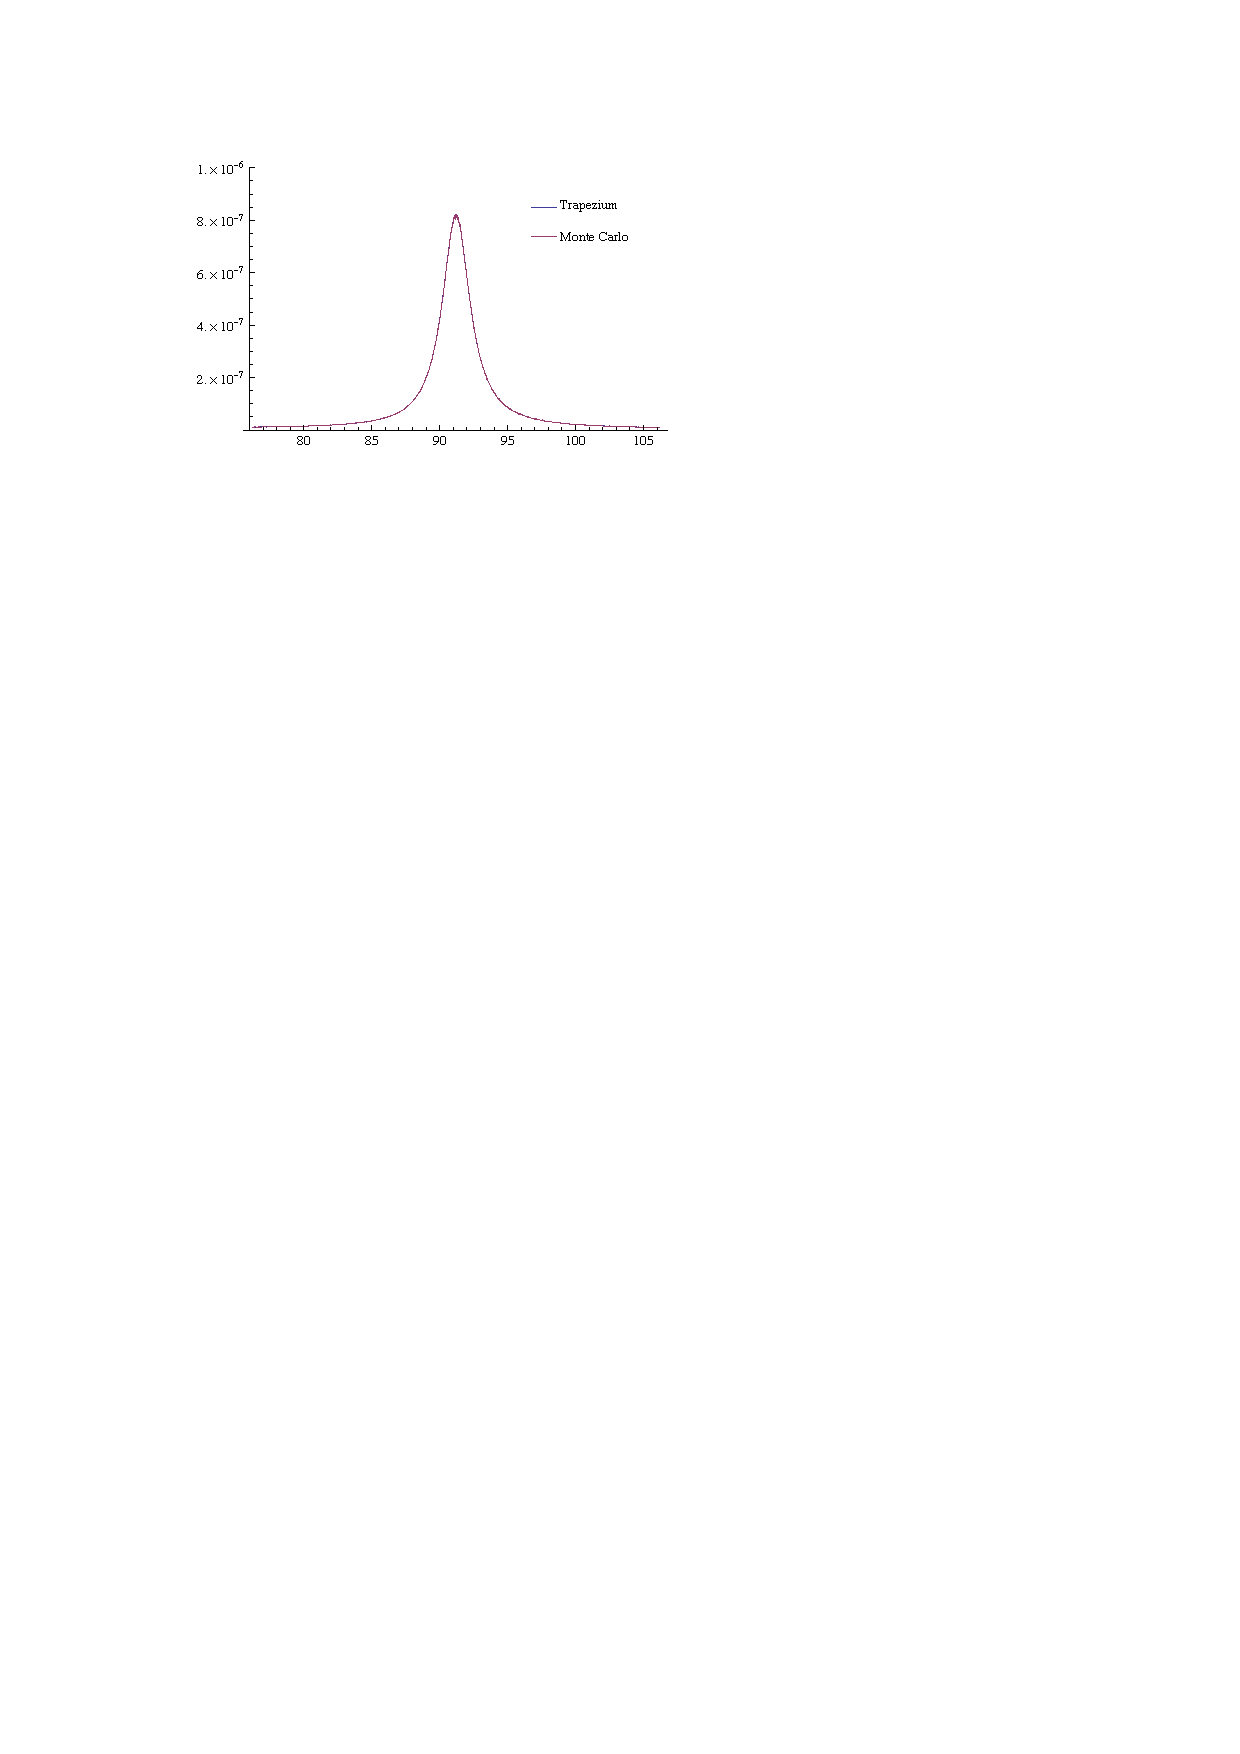
\includegraphics[width=1.2\textwidth]{both_combined_focused}
	\caption{Trapezium and Montecarlo cross section $\sigma$ for collider energies centred $15\GeV$ around $M_{\Zzero}$.}
	\label{fig:bothfocused}
\end{figure}

\begin{figure}[H]
	\vspace{10pt}
	\hspace*{-0.2\textwidth}
	\centering
	\subfloat[Trapezium]{
		\label{fig:trapgammaz}
		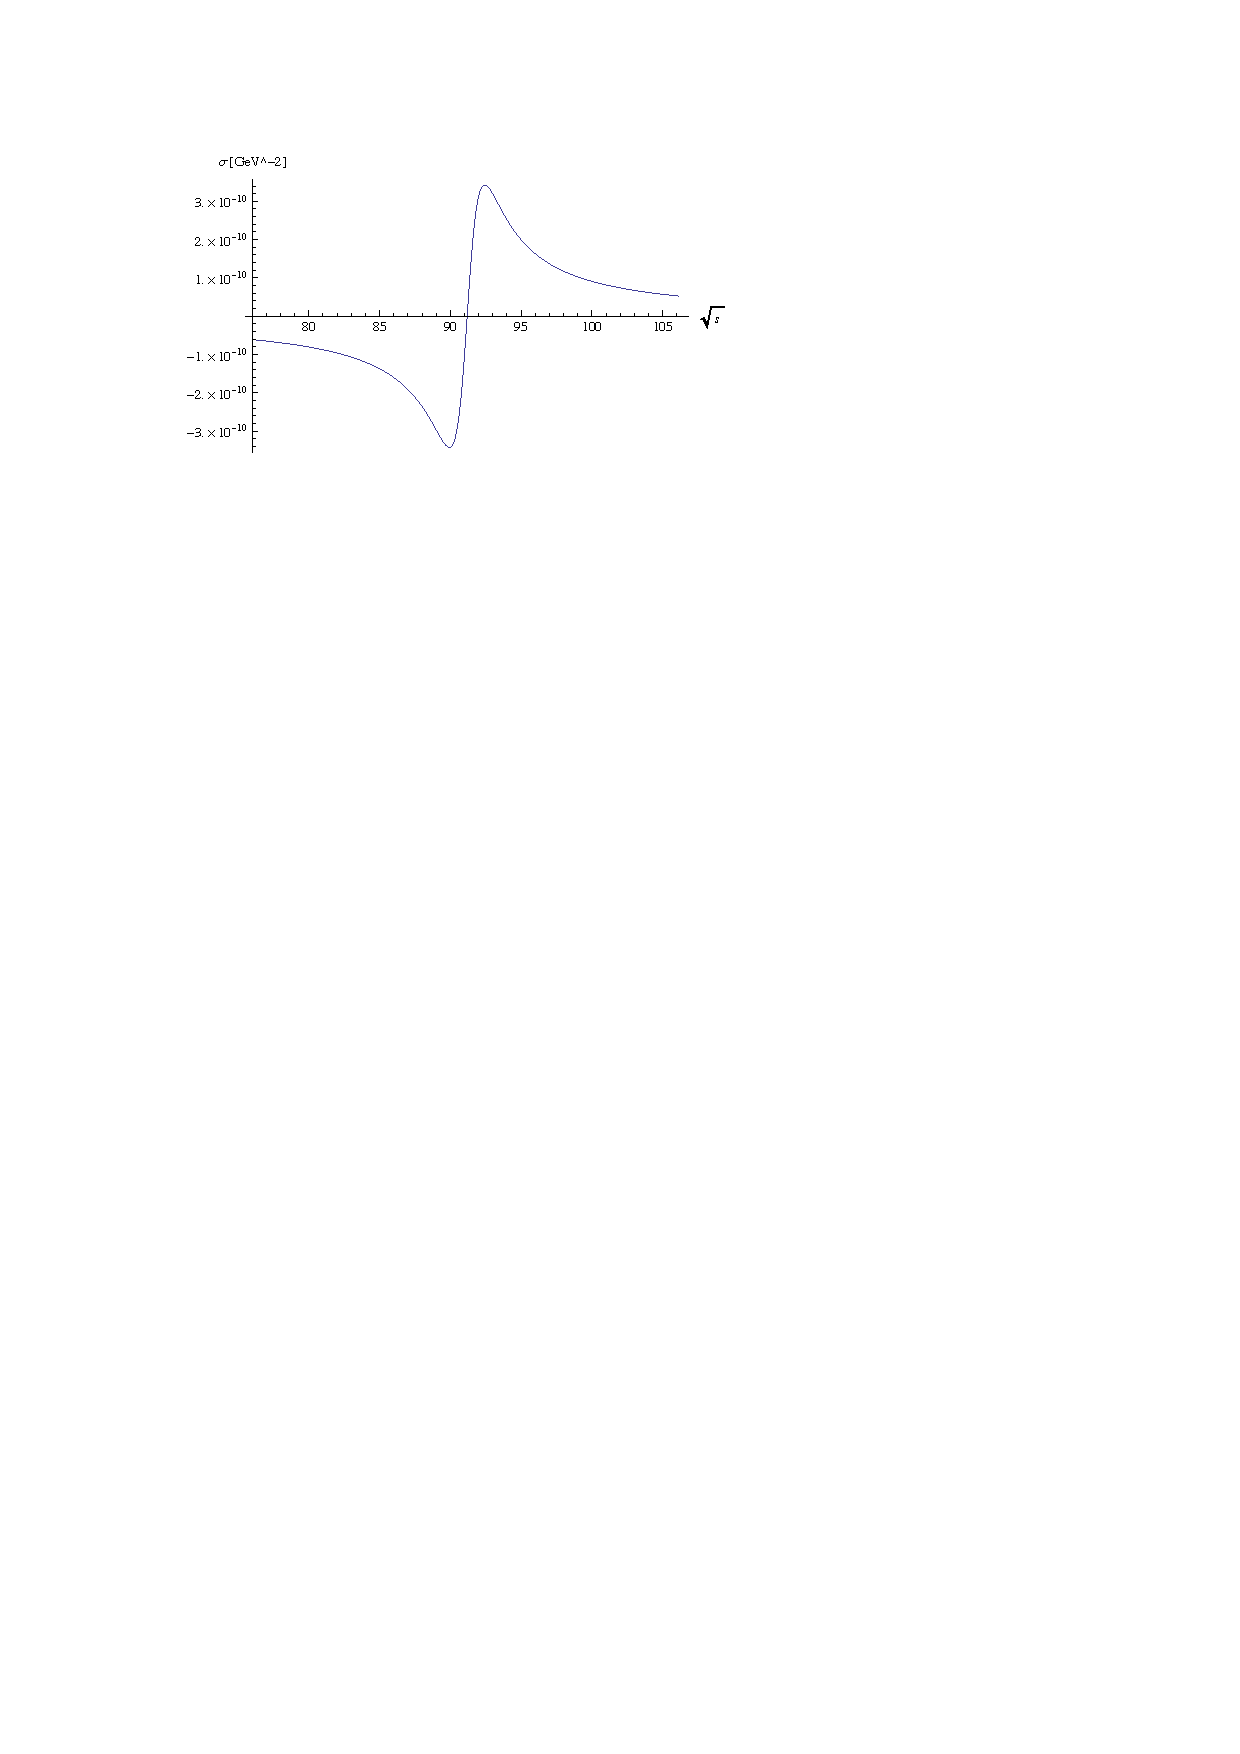
\includegraphics[width=0.7\textwidth]{trap_gamma_z}
	}
	\subfloat[Monte Carlo with trapezium superimposed]{
		\label{fig:mcgammaz}
		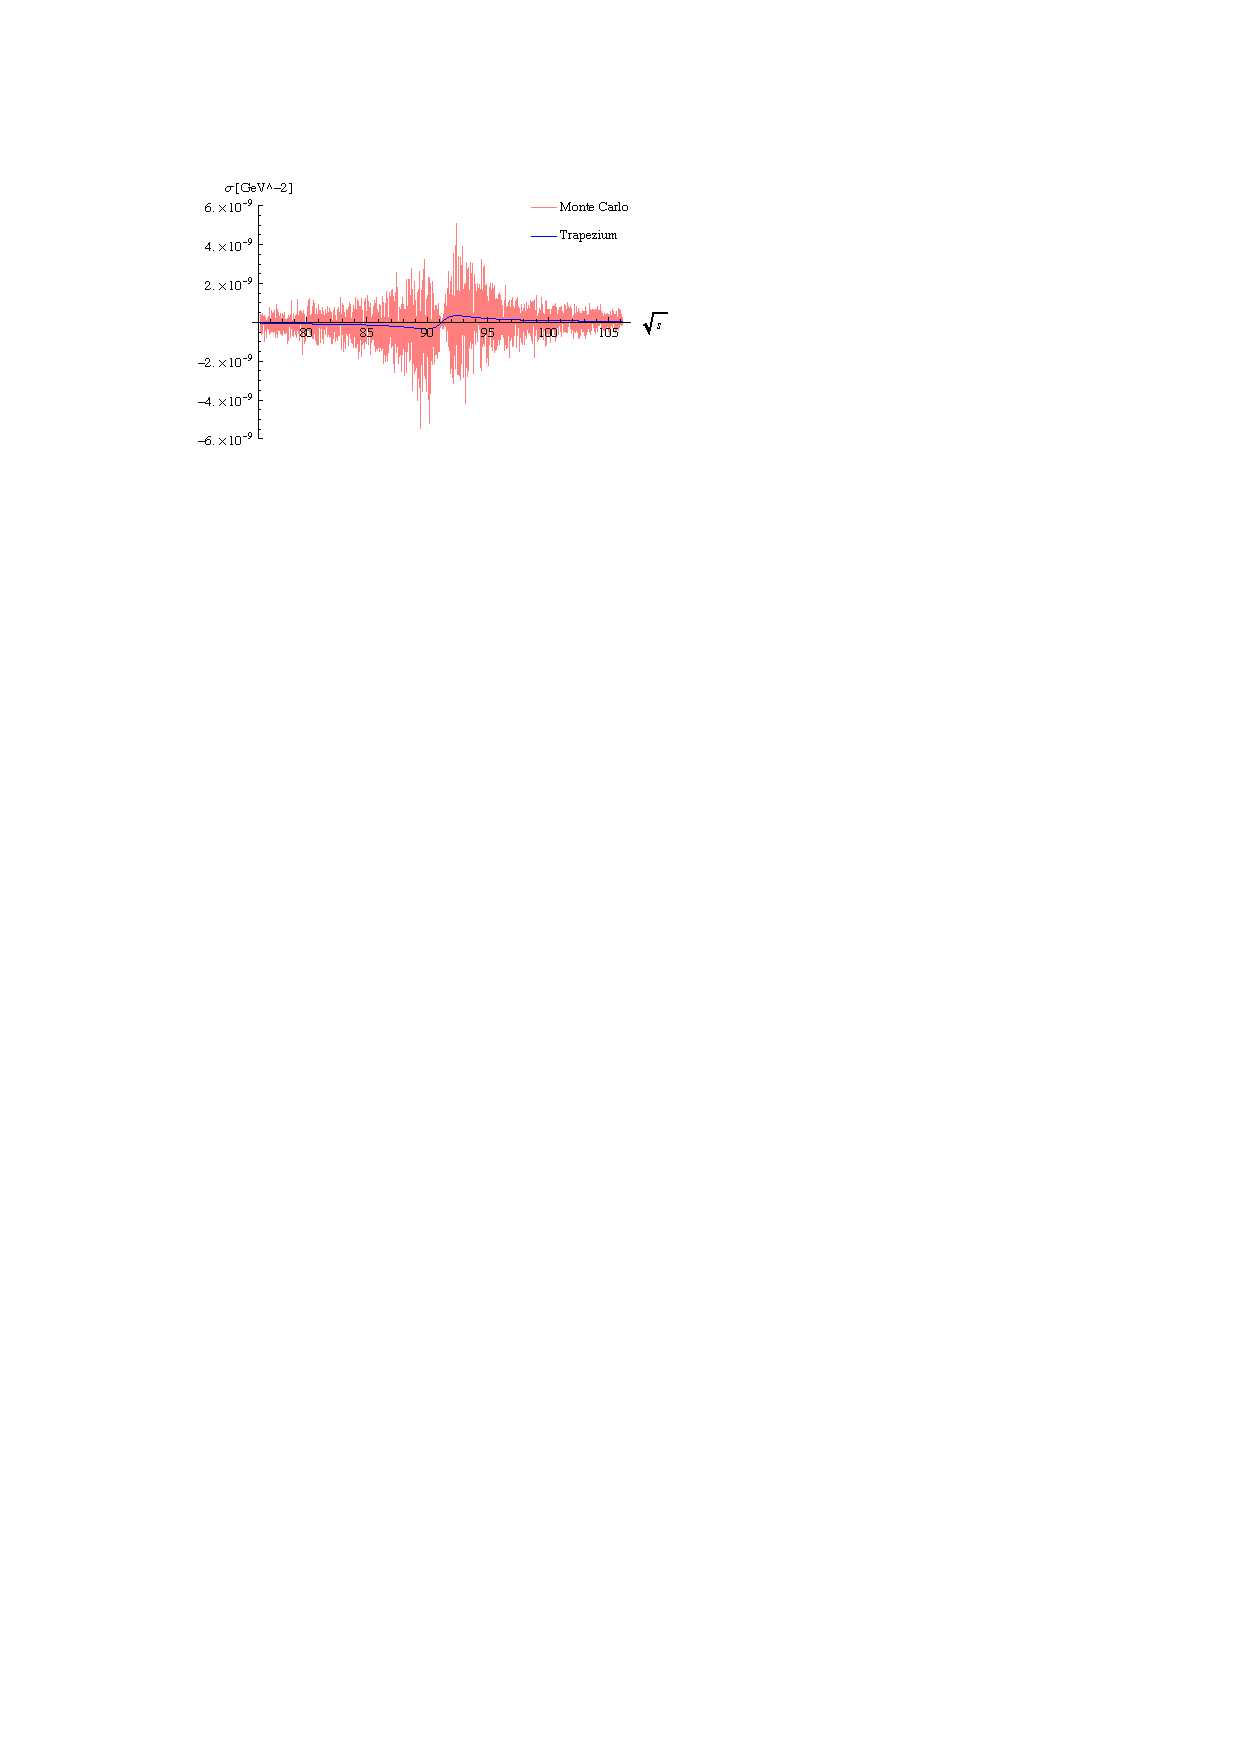
\includegraphics[width=0.7\textwidth]{both_gamma_z}
	}
	\caption{$\gamma\operatorname{-}\Zzero$ cross section for collider energies centred $15\GeV$ around $M_{\Zzero}$.}
	\label{fig:bothgammaz}
\end{figure}

\begin{figure}[H]
	\vspace{10pt}
	\hspace*{-0.1\textwidth}
	\centering
	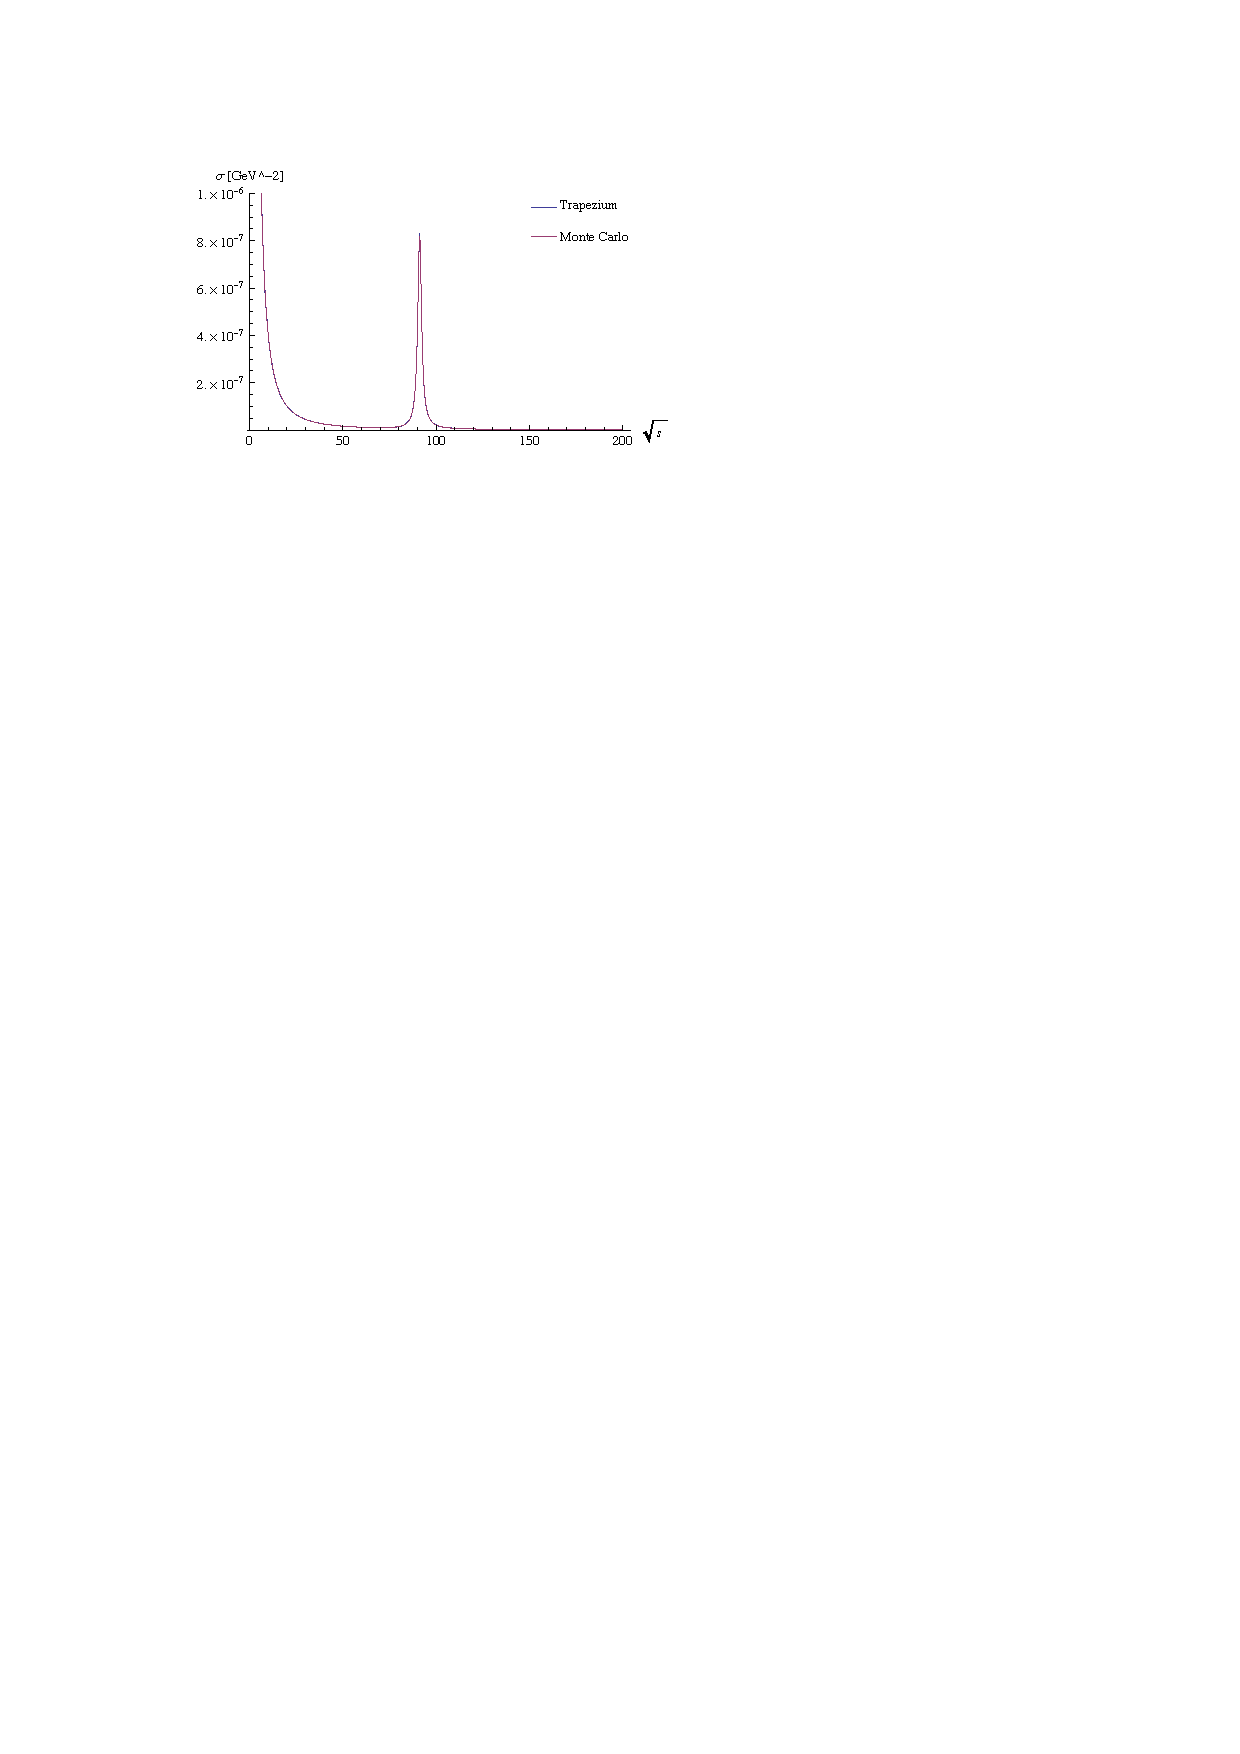
\includegraphics[width=1.2\textwidth]{c_both}
	\caption{Trapezium and Montecarlo cross section $\sigma$ for collider energies from $3\GeV$ to $200\GeV$. This data was produced by a C script, whereas all other plots use data from a Python script.}
	\label{fig:cboth}
\end{figure}

\newpage

\appendix
\section{Differential Cross Sections}\label{app:differentials}

The cross sections corresponding to the photon, $\Zzero$, and interference matrix elements follow. Due to the length of the analytic solutions, constants are defined, then the cross section is defined with respect to these constants. The differentials are given by G J Daniell~\cite{ref:gjdaniell}.

The small energy scales that will be reachable at LEP allow us to take the couplings $g_{e}$ and $g_{z}$ as constant. We define $g_{e}=\sqrt{4\pi\alpha}$ and $g_{z}=\sqrt{4\pi\alpha}(\cos{\theta_{w}}\sin{\theta_{w}})^{-1}$.\footnote{$\alpha$ is taken to be $\frac{1}{128}$, $\sin^{2}{\theta_{w}}$ is taken to be $0.23152$.}

\subsection{$\gamma\operatorname{-}\gamma$}

Define
$$
\alpha = \frac{g_{e}^{4}}{(8\pi)^{2}s} \sqrt{1-4\varepsilon^{2}}.
$$
Then

$$
\frac{\d{\sigma}}{\d{\Omega}}^{\gamma\operatorname{-}\gamma} = \alpha (1 + \cos^{2}{\vartheta} + 4\varepsilon^{2}\sin^{2}{\vartheta}),
$$
\begin{equation}
\sigma^{\gamma\operatorname{-}\gamma} = \frac{16\pi\alpha}{3}(1 + 2\varepsilon^{2}).
\end{equation}

\subsection{$\Zzero\operatorname{-}\Zzero$}

Define
\begin{align*}
\alpha &= \frac{g_{\Zzero}^{4}}{(32\pi)^{2}s} \frac{\sqrt{1-4\varepsilon^{2}}}{(1-\lambda^{2})^{2} + (\frac{\lambda\GZ}{\rts})},
\\
\beta &= ((C_{V}^{e})^{2} + (C_{A}^{e})^{2})((C_{V}^{\mu})^{2}),
\\
\Gamma &= ((C_{V}^{e})^{2} + (C_{A}^{e})^{2})((C_{A}^{\mu})^{2})(1-4\varepsilon^{2}),
\\
\Delta &= 8C_{V}^{e}C_{A}^{e}C_{V}^{\mu}C_{A}^{\mu}\sqrt{1-4\varepsilon^{2}}.
\end{align*}
Then

$$
\frac{\d{\sigma}}{\d{\Omega}}^{\Zzero-\Zzero}
  = \alpha(\beta(1+\cos^{2}{\vartheta}+4\varepsilon^{2}\sin^{2}{\vartheta})
    + \Delta(1+\cos^{2}{\vartheta})
    + \Gamma\cos{\vartheta}
  ),
$$
\begin{equation}
\sigma^{\gamma\operatorname{-}\gamma} = \frac{16\pi\alpha}{3}(\Gamma + (1 + 2\varepsilon^{2})\beta).
\end{equation}

\subsection{$\gamma\operatorname{-}\Zzero$}

Define
\begin{align*}
\alpha &= \frac{g_{\Zzero}^{4}}{(32\pi)^{2}s} \frac{\sqrt{1-4\varepsilon^{2}}}{(1-\lambda^{2})^{2} + (\frac{\lambda\GZ}{\rts})},
\\
\beta &= ((C_{V}^{e})^{2} + (C_{A}^{e})^{2})((C_{V}^{\mu})^{2}),
\\
\Gamma &= ((C_{V}^{e})^{2} + (C_{A}^{e})^{2})((C_{A}^{\mu})^{2})(1-4\varepsilon^{2}),
\\
\Delta &= 8C_{V}^{e}C_{A}^{e}C_{V}^{\mu}C_{A}^{\mu}\sqrt{1-4\varepsilon^{2}}.
\end{align*}
Then

$$
\frac{\d{\sigma}}{\d{\Omega}}^{\gamma-\Zzero}
  = \alpha(\beta(1+\cos^{2}{\vartheta}+4\varepsilon^{2}\sin^{2}{\vartheta})
    + \Delta\cos{\vartheta}
  ),
$$
\begin{equation}
\sigma^{\gamma-\Zzero} = \frac{16\pi\alpha\beta}{3}(1 + 2\varepsilon^{2}).
\end{equation}

\begin{thebibliography}{9}
	\bibitem{ref:wpaper}
  G. Arnison et al.,
  ``Experimental observation of isolated large transverse energy electrons with associated missing energy at $\sqrt{s}=540\GeV$,''
  \emph{\PL}\textbf{122B},
  Issue 1,
  p103-116 (1983).
  
	\bibitem{ref:zpaper}
  G. Arnison et al.,
  ``Experimental observation of lepton pairs of invariant mass around 95 $\GeV/c^{2}$ at the CERN SPS collider,''
  \emph{\PL}\textbf{126B},
  Issue 5,
  p398-410 (1983).

  \bibitem{ref:gjdaniell}
  G. J. Daniell,
  \emph{PHYS6017 Course Notes},
  2011.
  
  \bibitem{ref:dgriffiths}
  D. Griffiths,
  \emph{Introduction to Elementary Particles},
  Wiley-VCH, Weinheim,
  6th Edition,
  2011.
  
  \bibitem{ref:pdg}
  K. Nakamura et al. (Particle Data Group),
  J.{} Phys.{} G \textbf{37},
  075021 (2010) and 2011 partial update for the 2012 edition.
\end{thebibliography}
 
\end{document}